% Draft thesis. Replace this preamble and the front matter with the department's
% LaTeX template when it is available; the chapter files can be \input unchanged.
\documentclass[12pt,a4paper,oneside]{report}
\usepackage[T1]{fontenc}
\usepackage[margin=2.5cm]{geometry}
\usepackage{graphicx,booktabs,tabularx,amsmath,amssymb,siunitx,caption,float}
\usepackage[hidelinks]{hyperref}
\usepackage[numbers,sort&compress]{natbib}
\graphicspath{{../reports/figures/}{figures/}}
\setlength{\parskip}{4pt}
\newcolumntype{Y}{>{\raggedright\arraybackslash}X}

\begin{document}
\title{Three-Year Dementia Risk Prediction from Multimodal NACC Data:\
Does Cardiovascular Information Add Value Beyond Cognition?}
\author{Team names and roll numbers}
\date{October 2026}
\maketitle

\tableofcontents
\listoffigures
\listoftables

\chapter{Introduction}
\textit{To be written (see docs/thesis\_outline.md).}

\chapter{Literature Review}
\textit{To be written (see docs/thesis\_outline.md).}

\chapter{Data}
\label{ch:data}

\section{The National Alzheimer's Coordinating Center}

The study uses the Freeze~74 release (June 2026) of the National Alzheimer's Coordinating Center (NACC) database. NACC pools longitudinal data from Alzheimer's Disease Research Centers across the United States. Volunteers are assessed roughly once a year with the Uniform Data Set (UDS), a fixed battery of questionnaires, examinations and neuropsychological tests that every centre administers in the same way \cite{weintraub2018}. The release used here contains 217,598 visits from 57,038 participants at 46 centres, collected between June 2005 and May 2026. Participants are referred through memory clinics or volunteer directly, so the cohort is a research sample and not a population sample: at the first visit the median age is 71 years, median education is 16 years and 76\% of participants identify as White.

Access to the data is governed by the NACC data use agreement. All analysis was performed on a local machine. No participant-level value, identifier or image file name appears in this thesis, in the code repository or in any shared report; every reported number is an aggregate.

\section{Files received}

Table~\ref{tab:files} lists the ten tables in the release. Only the main clinical table and the four summary PET tables contribute model inputs; the remaining files were audited but do not supply features.

\begin{table}[H]
\centering\small
\caption{Files in the NACC release and their role in this study.}
\label{tab:files}
\begin{tabularx}{\textwidth}{@{}lrrY@{}}
\toprule
File & Rows & Participants & Role \\
\midrule
Main clinical table (\texttt{ftldlbd}) & 217,598 & 57,038 & All clinical features and the outcome \\
SCAN amyloid PET summary & 3,933 & 3,566 & Centiloids and amyloid status \\
Mixed-protocol amyloid PET summary & 2,235 & 2,073 & Same, for older scans \\
SCAN tau PET & 2,653 & 2,405 & Meta-temporal and entorhinal SUVR \\
Mixed-protocol tau PET & 671 & 616 & Same, for older scans \\
SCAN and mixed-protocol amyloid PET, regional & 6,168 & --- & Not used (tracer-specific SUVR) \\
SCAN FDG PET & 885 & 639 & Not used (about 600 linked participants) \\
SCAN PET quality-control list & 8,759 & 4,585 & Audit of the local image folders \\
CLARiTI study tracking & 857 & 776 & Not used (administrative) \\
\bottomrule
\end{tabularx}
\end{table}

In the clinical table one row is one visit; in the PET tables one row is one scan. The participant identifier is the only key shared by all tables. Because a scan is not tied to a visit number, each scan has to be matched to a visit by date (Section~\ref{sec:pettiming}).

In addition, 599 raw PET acquisitions (318 amyloid, 232 tau and 49 FDG scans from 446 participants, about 100\,GB of DICOM files) were available locally. They are used in Chapter~\ref{ch:petimages}.

\section{The clinical table}

The clinical table has 2,649 columns, but most of them are empty for most visits: modules for frontotemporal and Lewy body disease, autopsy findings, form version~4 items and free text. Only 787 columns contain data in at least 10\% of visits. From these, 114 variables were mapped by hand to a meaning, a category, a role and their own missing-value codes, following the NACC Researcher's Data Dictionary. Seventy-six of them are used to build the model inputs.

\subsection{Missing-value codes}

NACC encodes non-responses with numeric codes whose meaning depends on the variable: $-4$ marks a question that was not part of the visit, codes such as 8, 88 or 888 mark ``not applicable'', and 9, 99 or 999 mark ``unknown''. These codes cannot be removed globally. The value 88, for example, is a genuine age in 3,655 visits and a genuine diastolic pressure in 3,090 visits, but means ``never smoked'' in the years-smoked column (73,669 visits). Cleaning was therefore performed column by column from the variable map.

\subsection{Changes in the forms}

The UDS has been revised three times. The most important change for this study took place with version~3 in 2015, when the neuropsychological battery was replaced: the MMSE, Logical Memory, Digit Span and Boston Naming tests were replaced by the MoCA, Craft Story, Number Span and MINT tests. Only category fluency and the Trail Making tests are common to all versions. The same participant can therefore have different tests at different visits. Health history is also recorded on two forms: the participant-reported history (form A5) and, in version~3, the clinician-assessed conditions (form D2). Telephone visits contain no neuropsychological tests. Figure~\ref{fig:tests} shows how the availability of each test changes between versions; it is the reason the tests were converted into common domain scores (Section~\ref{sec:zscores}).

\begin{figure}[H]
\centering
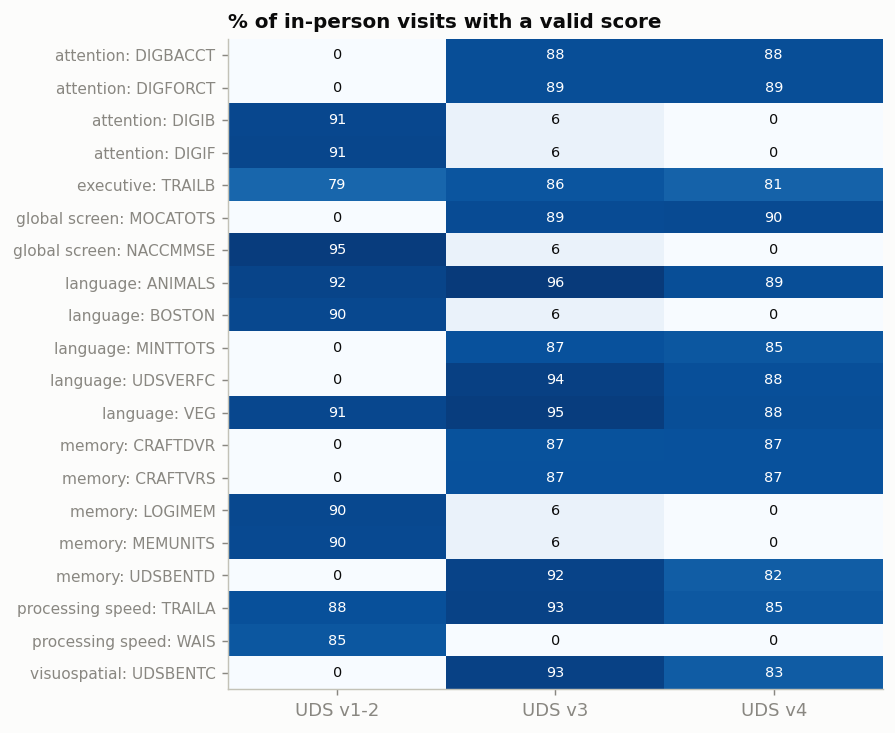
\includegraphics[width=0.8\textwidth]{03_test_availability.png}
\caption{Percentage of in-person visits with a valid score for each neuropsychological test, by UDS version. Tests of versions 1--2 and of version~3 are almost disjoint.}
\label{fig:tests}
\end{figure}


\section{Feature categories}

The variables used are grouped into five categories (Table~\ref{tab:categories}). The complete list, with source columns and value codes, is given in Appendix~A.

\begin{table}[H]
\centering\small
\caption{Feature categories, source columns and number of model features.}
\label{tab:categories}
\begin{tabularx}{\textwidth}{@{}lYr@{}}
\toprule
Category & Main source columns & Features \\
\midrule
Demographics & \texttt{NACCAGE}, \texttt{NACCSEX}, \texttt{EDUC}, \texttt{NACCNIHR}, \texttt{NACCHISP}, \texttt{NACCLIVS} & 8 \\
Cardiovascular and medical & Twelve conditions from forms A5 and D2, smoking, blood pressure, heart rate, BMI, four medication classes and the medication count & 25 \\
Cognitive tests & Twenty neuropsychological tests, the Geriatric Depression Scale and twelve NPI-Q behaviour items & 9 \\
Clinical stage & \texttt{CDRSUM}, \texttt{NACCUDSD} & 3 \\
Genetics & \texttt{NACCNE4S}, \texttt{NACCFAM} & 3 \\
PET (second-stage model only) & \texttt{CENTILOIDS}, amyloid status, meta-temporal and entorhinal tau SUVR & 4 \\
\bottomrule
\end{tabularx}
\end{table}

Four groups of variables were deliberately excluded. Autopsy findings are known only after death and would leak future information. The Functional Activities Questionnaire, the level of independence, subjective and informant-reported memory complaints and the use of Alzheimer's medication are so close to the diagnosis itself that including them would partly reproduce the clinician's decision; they were evaluated separately as a sensitivity analysis. Regional PET values were not used because they are tracer-specific and highly redundant. Form version~4 visits (3\% of visits) were excluded because they use new variable names.

\section{PET data}
\label{sec:petdata}

Amyloid PET values are available for about 5,100 participants who also appear in the clinical table, and tau PET values for 2,724. The amyloid tables provide the Centiloid value, which is comparable across tracers, and a positive or negative status assigned by the PET core. The tau tables provide standardised uptake value ratios (SUVR) in about 160 regions; the meta-temporal composite and the entorhinal cortex were retained as the standard summaries of early tau deposition. Because the two tau tracers (flortaucipir and MK-6240) give different SUVR scales, each tau value was standardised within tracer against amyloid-negative participants from the training set. Only scans that passed quality control were used.

Most PET scans are recent, so few scanned participants have three years of clinical follow-up after the scan. This limits what can be learned from PET in this cohort (Section~\ref{sec:res_pet}).

\chapter{Methodology}
\label{ch:method}

\section{Prediction task}

The prediction is made at an \emph{index visit}, using only information available at or before that visit. For a participant without dementia at the index visit, the task is to estimate the probability of a clinical diagnosis of dementia within three years:
\begin{equation}
\hat{p} = P\left(\text{dementia diagnosed in } (t_0, t_0 + 3\ \text{years}] \mid \mathbf{x}_{t_0}\right),
\end{equation}
where $t_0$ is the date of the index visit and $\mathbf{x}_{t_0}$ the feature vector at that visit. The main analysis uses each participant's first visit as the index visit. If $T$ denotes the time from $t_0$ to the first visit with a dementia diagnosis and $C$ the time to the last visit, the binary label is
\begin{equation}
y = \begin{cases}
1 & \text{if } T \le 3, \\
0 & \text{if } T > 3 \text{ and } C \ge 3, \\
\text{unknown} & \text{if } T > 3 \text{ and } C < 3,
\end{cases}
\end{equation}
with times in years.

\subsection{Choice of horizon and outcome}

Clinical diagnosis (\texttt{NACCUDSD}) and the Clinical Dementia Rating are recorded at every visit in every form version, which makes them the most consistent outcomes available. A dementia diagnosis was chosen as the main outcome because it is clinically meaningful and easy to interpret. The three-year horizon balances the number of events against loss to follow-up: Kaplan--Meier estimates \cite{kaplan1958} show that about 35\% of participants with MCI progress to dementia within three years, and that 11\% of cognitively normal participants progress to MCI or dementia, while the number of participants with a known status falls steadily with longer horizons and most PET scans are too recent for a five-year horizon. The Kaplan--Meier estimate of the probability of remaining free of the event up to time $t$ is
\begin{equation}
\hat{S}(t) = \prod_{t_i \le t} \left(1 - \frac{d_i}{n_i}\right),
\end{equation}
where $d_i$ is the number of events at time $t_i$ and $n_i$ the number of participants still under observation just before $t_i$; the three-year progression rate is $1 - \hat{S}(3)$ (Figure~\ref{fig:km}).

\begin{figure}[H]
\centering
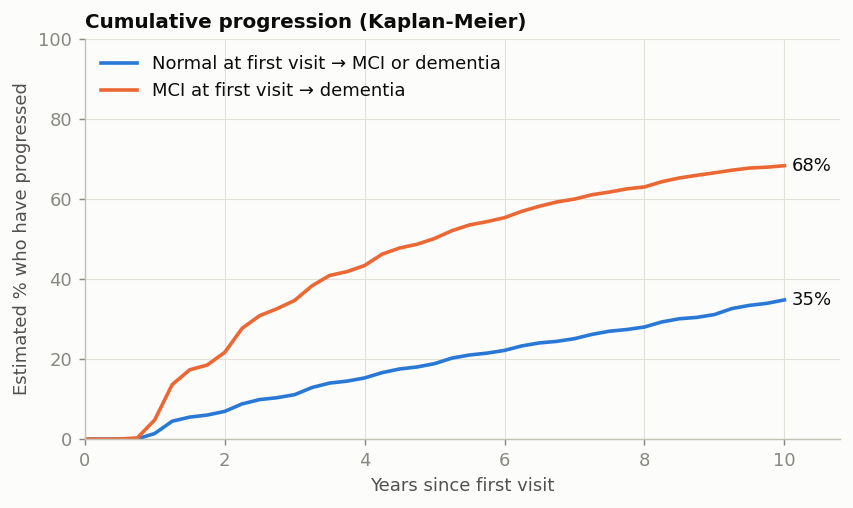
\includegraphics[width=0.75\textwidth]{02_progression_curves.png}
\caption{Kaplan--Meier estimates of cumulative progression from the first visit: cognitively normal participants to MCI or dementia, and participants with MCI to dementia.}
\label{fig:km}
\end{figure}


\subsection{Censoring}

A participant last seen less than three years after the index visit without a dementia diagnosis has an unknown outcome. Such participants were excluded from the binary task rather than counted as negative, which would bias the estimated risk downwards. Because this exclusion could itself introduce bias, a Cox proportional hazards model \cite{cox1972} that uses all eligible participants, including the censored ones, was fitted as a robustness check (Section~\ref{sec:res_sens}). Figure~\ref{fig:outcome} illustrates the three possible cases.

\begin{figure}[H]
\centering
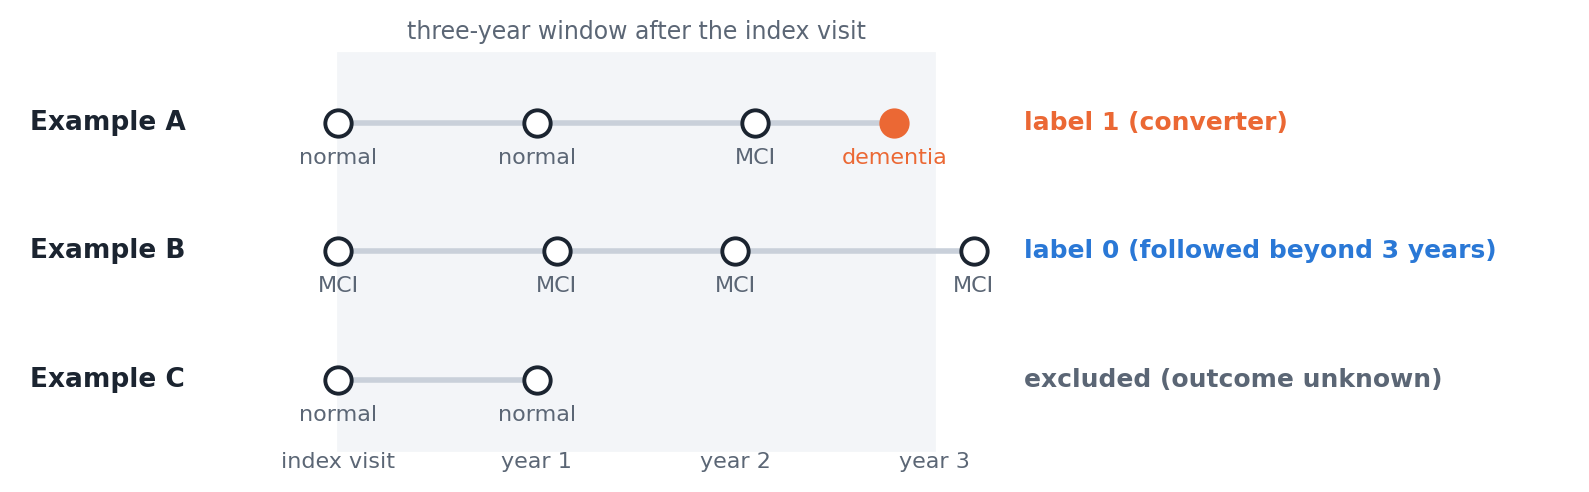
\includegraphics[width=\textwidth]{outcome.png}
\caption{Definition of the outcome. Only the index visit supplies features; later visits supply the label.}
\label{fig:outcome}
\end{figure}

\subsection{Secondary outcomes: cognitive decline}

Dementia is one end point of cognitive decline, but many people worsen without reaching it. Two further outcomes were therefore defined from the CDR Sum of Boxes, which is recorded at every visit in every form version. The binary decline outcome is a rise of at least one point in CDR-SB at any visit within three years of the index visit; it is unknown for participants who neither rose by a point nor were followed for three years. The continuous progression outcome is the change in CDR-SB between the index visit and the visit closest to three years later, accepted if that visit falls within six months of the three-year mark. Writing $c(t)$ for CDR-SB at time $t$ after the index visit and $v_i$ for the visit times,
\begin{equation}
y_{\text{dec}} = \mathbb{1}\Big[\max_{0 < v_i \le 3} c(v_i) - c(0) \ge 1\Big],
\qquad
\Delta = c(v^{*}) - c(0), \quad v^{*} = \operatorname*{arg\,min}_{|v_i - 3| \le 0.5} |v_i - 3|.
\end{equation}
The same eligibility rules and splits are used for all outcomes.

\section{Cohort}

Table~\ref{tab:flow} shows how the cohort was formed. Visits had to be in person, because telephone visits lack the neuropsychological tests, and on form versions 1 to 3, because version~4 reorganised many of the other variables and accounts for only 3\% of visits. Participants with dementia at the index visit, or at any earlier visit, are not eligible.

\begin{table}[H]
\centering\small
\caption{Cohort flow.}
\label{tab:flow}
\begin{tabular}{@{}lr@{}}
\toprule
Step & Participants \\
\midrule
All participants & 57,038 \\
First visit in person, form version 1 to 3 & 55,461 \\
\quad and not demented at that visit & 38,107 \\
\quad and outcome known at three years & 19,470 \\
\quad\quad of whom diagnosed with dementia within three years & 2,818 (14.5\%) \\
\bottomrule
\end{tabular}
\end{table}

The ``not demented'' cohort contains three clinically different groups: 12,377 cognitively normal participants (198 converters, 1.6\%), 5,993 participants with MCI (2,485 converters, 41.5\%) and 1,100 participants classed as impaired but not MCI (135 converters, 12.3\%). Results are reported for the whole cohort and for the normal and MCI groups separately.

\section{Feature construction}

\subsection{Harmonised cognitive scores}
\label{sec:zscores}

To place tests from different form versions on one scale, each raw score $s$ was converted into a demographically adjusted $z$-score. For each test, a linear model of the score on age, sex and education was fitted among cognitively normal participants at their first visit, using the training set only:
\begin{equation}
\hat{s} = \beta_0 + \beta_1\,\text{age} + \beta_2\,\text{female} + \beta_3\,\text{education},
\qquad
z = \frac{s - \hat{s}}{\sigma_{\text{res}}},
\end{equation}
where $\sigma_{\text{res}}$ is the residual standard deviation of the fitted model. The sign is reversed for the two timed Trail Making tests, so that a negative $z$ always means worse than expected. Values were clipped to $[-5, 5]$. The $z$-scores of the tests in one cognitive domain were then averaged to give six domain scores: global screening (MoCA, MMSE), memory, attention, speed and executive function, language, and visuospatial function. A participant receives a domain score from whichever tests their visit contained.

As an example, for the MoCA the fitted model is $\hat{s} = 23.0 - 0.059\,\text{age} + 0.33\,\text{female} + 0.42\,\text{education}$ with $\sigma_{\text{res}} = 2.56$, estimated from 6,264 normal participants. A 72-year-old woman with 16 years of education has an expected score of 25.8, so a score of 21 corresponds to $z = -1.9$ (Figure~\ref{fig:zscore}).

\begin{figure}[H]
\centering
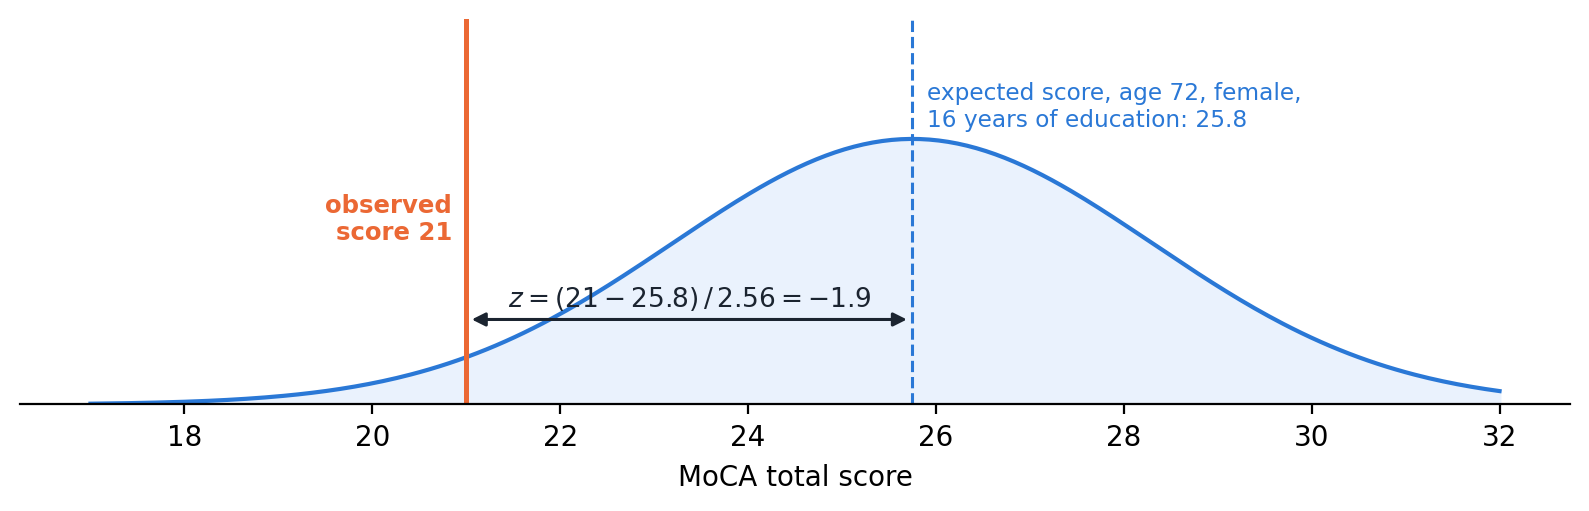
\includegraphics[width=\textwidth]{zscore.png}
\caption{Demographically adjusted $z$-score for the MoCA, using the fitted normative model.}
\label{fig:zscore}
\end{figure}

The harmonisation was checked on cognitively normal participants who were not used to fit the norms: their mean domain $z$-scores lie within 0.1 of zero under every form version, while participants with MCI and dementia score progressively lower (Figure~\ref{fig:harmon}). The scores therefore mean the same thing whichever tests a visit contained.

\begin{figure}[H]
\centering
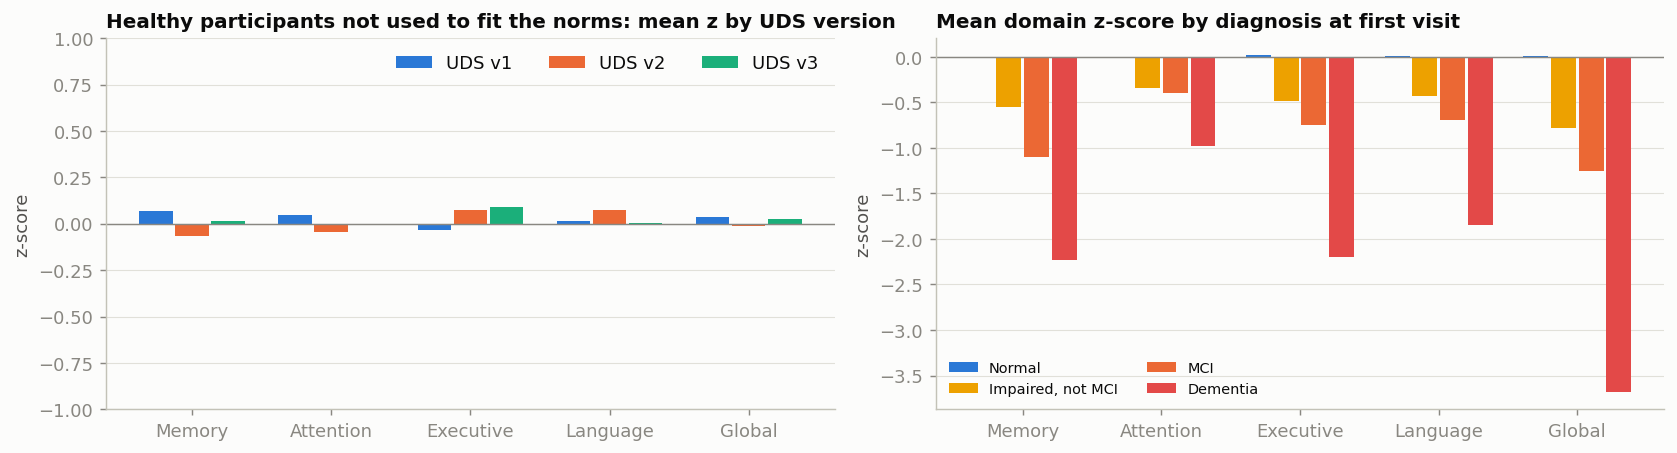
\includegraphics[width=\textwidth]{05_cognitive_harmonisation.png}
\caption{Left: mean domain $z$-score of cognitively normal participants not used to fit the norms, by UDS version. Right: mean domain $z$-score by diagnosis at the first visit.}
\label{fig:harmon}
\end{figure}


Three further cognitive features were derived: the number of tests the participant could not complete for cognitive or behavioural reasons (NACC code 96 or 996), which is informative about severity and is therefore kept rather than treated as missing; the Geriatric Depression Scale total; and the number of NPI-Q behavioural symptoms present.

\subsection{Cardiovascular history}

Each condition $k$ was coded as ``ever present'', $h_k(t) = \max_{v_i \le t} r_k(v_i)$, where $r_k(v_i) = 1$ if the condition is recorded at visit $v_i$. The record was taken from the participant-reported history (form A5, where both recent and remote mentions count) and, where that form was blank, from the clinician-assessed form D2. Once present, a condition remains present at all later visits. Measured blood pressure, heart rate and BMI use the most recent measurement up to the visit. Two summary features were derived: pulse pressure, $\text{PP} = \text{BP}_{\text{sys}} - \text{BP}_{\text{dia}}$, and the vascular risk count, $R = h_{\text{HTN}} + h_{\text{chol}} + h_{\text{DM}} + h_{\text{smoke}} \in \{0, \dots, 4\}$.

\subsection{Genetics}

The number of APOE $\varepsilon$4 alleles is used directly. About one participant in five was not genotyped; genotyping depends on centre and consent and is therefore not random, so these participants receive a separate ``not genotyped'' indicator instead of an imputed value.

\subsection{Preventing the use of future information}
\label{sec:pettiming}

No feature at a visit may depend on a later visit. Fixed characteristics such as education are carried forward from the visit where they were first recorded, never backwards. A PET scan is used at a visit only if it was acquired on or up to 365 days before that visit. Both rules were introduced after the verification step described in Chapter~\ref{ch:verification} found violations in an earlier version of the pipeline.

\section{Data splits}

All splits were made at participant level, so that all visits of a person fall in the same partition. Twenty percent of the centres (9 of 46) were held out entirely to measure performance at sites the model has never seen. The remaining participants were divided into training (70\%), validation (15\%) and test (15\%) sets, stratified by diagnosis at the first visit. The random seed was fixed (2026). Table~\ref{tab:splits} gives the resulting sizes for the first-visit cohort.

\begin{table}[H]
\centering\small
\caption{Partition sizes for the main cohort.}
\label{tab:splits}
\begin{tabular}{@{}lrr@{}}
\toprule
Partition & Participants & Converters \\
\midrule
Training & 10,879 & 1,599 \\
Validation & 2,241 & 342 \\
Test & 2,286 & 332 \\
Held-out centres & 4,064 & 545 \\
\bottomrule
\end{tabular}
\end{table}

\begin{figure}[H]
\centering
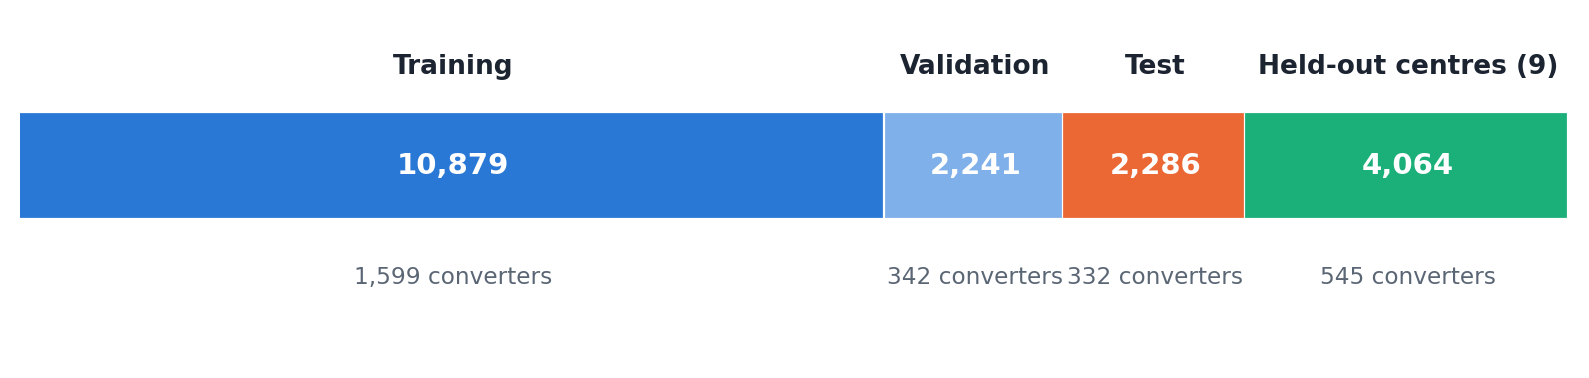
\includegraphics[width=\textwidth]{split.png}
\caption{Participant-level partitions of the main cohort.}
\label{fig:split}
\end{figure}

Every quantity estimated from data (normative models for $z$-scores, tau standardisation, imputation medians, scaling) was fitted on the training set and applied unchanged to the other sets. The validation set was used for early stopping and model selection; the test set and the held-out centres were used only for evaluation.

\section{Models}

Five classifiers of increasing complexity were compared on the same 48 features (Table~\ref{tab:models}); their mathematical form is given in Section~\ref{sec:model_maths}. Logistic regression is the standard baseline in clinical prediction. Random forests \cite{breiman2001} and gradient-boosted trees (XGBoost \cite{chen2016}) are strong learners for tabular data that handle non-linear effects and interactions. A multilayer perceptron and the FT-Transformer \cite{gorishniy2021} represent deep learning; the latter tokenises each feature and applies self-attention, and is among the strongest deep architectures reported for tabular data. Except for logistic regression, every model was trained with three random seeds and the predictions were averaged.

\begin{table}[H]
\centering\small
\caption{Models and settings.}
\label{tab:models}
\begin{tabularx}{\textwidth}{@{}lY@{}}
\toprule
Model & Settings \\
\midrule
Logistic regression & Median imputation with missing-value indicators, standardisation; regularisation strength chosen from five values on the validation set \\
Random forest & 500 trees, minimum 10 samples per leaf, $\sqrt{p}$ features per split \\
XGBoost & Up to 3,000 trees, learning rate 0.03, depth chosen from \{3, 4, 6\} on validation AUROC, subsample and column sample 0.8, early stopping after 100 rounds without improvement; missing values handled natively \\
Multilayer perceptron & Two hidden layers (128 and 64 units), dropout 0.2, AdamW, early stopping on validation AUROC \\
FT-Transformer & Feature tokens of dimension 64, three Transformer layers with eight heads, a learned token for each missing feature, early stopping on validation AUROC \\
\bottomrule
\end{tabularx}
\end{table}

XGBoost was used as the main model for all further experiments because it performed as well as the others, handles missing values without imputation and allows exact Shapley value explanations. For the progression outcome, the same gradient-boosting settings were used with an absolute-error objective, and the model was compared with the simplest reference, predicting no change.

\subsection{Mathematical form of the models}
\label{sec:model_maths}

Let $\mathbf{x} \in \mathbb{R}^{p}$ be the feature vector of a participant, $y \in \{0,1\}$ the label and $\sigma(u) = 1/(1+e^{-u})$ the logistic function. All classifiers output a probability $\hat{p} = \sigma(f(\mathbf{x}))$ and, apart from the random forest, are fitted by minimising the binary cross-entropy over the $n$ training participants,
\begin{equation}
\mathcal{L}_{\text{BCE}} = -\frac{1}{n} \sum_{i=1}^{n} \Big[ y_i \log \hat{p}_i + (1 - y_i) \log (1 - \hat{p}_i) \Big],
\label{eq:bce}
\end{equation}
plus a model-specific penalty.

\paragraph{Logistic regression.} After median imputation, missing-value indicators and standardisation give a vector $\tilde{\mathbf{x}}$, the model is $f(\mathbf{x}) = \beta_0 + \boldsymbol{\beta}^{\top}\tilde{\mathbf{x}}$ with an $L_2$ penalty,
\begin{equation}
\min_{\beta_0, \boldsymbol{\beta}} \; \frac{1}{2}\lVert \boldsymbol{\beta} \rVert_2^2 + C \sum_{i=1}^{n} \ell(y_i, \hat{p}_i), \qquad C \in \{0.01, 0.03, 0.1, 0.3, 1\},
\end{equation}
where $\ell$ is the per-participant cross-entropy and $C$ was chosen on the validation set.

\paragraph{Random forest.} The forest averages the class-probability estimates of $B = 500$ decision trees, each grown on a bootstrap sample with $\lfloor\sqrt{p}\rfloor$ candidate features per split: $\hat{p}(\mathbf{x}) = \frac{1}{B}\sum_{b=1}^{B} \hat{p}_b(\mathbf{x})$.

\paragraph{Gradient-boosted trees (XGBoost).} The score is a sum of regression trees, built one at a time:
\begin{equation}
f_M(\mathbf{x}) = \sum_{m=1}^{M} \eta\, g_m(\mathbf{x}), \qquad \eta = 0.03.
\end{equation}
Tree $g_m$ is chosen to minimise a second-order approximation of the regularised objective
\begin{equation}
\sum_{i=1}^{n} \Big[ G_i\, g_m(\mathbf{x}_i) + \tfrac{1}{2} H_i\, g_m(\mathbf{x}_i)^2 \Big] + \gamma J + \tfrac{1}{2}\lambda \sum_{j=1}^{J} w_j^2,
\end{equation}
where $G_i = \hat{p}_i - y_i$ and $H_i = \hat{p}_i(1 - \hat{p}_i)$ are the first and second derivatives of the loss at the current model, $J$ is the number of leaves, $w_j$ the leaf values, $\lambda = 2$ and $\gamma = 0$. For a leaf containing the participant set $I_j$ the optimal value is $w_j^{*} = -\sum_{i \in I_j} G_i / (\sum_{i \in I_j} H_i + \lambda)$, and a split is kept only if every child has $\sum H_i \ge 5$ (minimum child weight). Missing values are sent down a default branch learned from the data. For the progression outcome the loss is the absolute error $\lvert \Delta_i - f(\mathbf{x}_i) \rvert$, whose minimiser is the conditional median.

\paragraph{Multilayer perceptron.} With $\tilde{\mathbf{x}}$ as for logistic regression,
\begin{equation}
\mathbf{h}_1 = \operatorname{ReLU}(\mathbf{W}_1 \tilde{\mathbf{x}} + \mathbf{b}_1), \quad
\mathbf{h}_2 = \operatorname{ReLU}(\mathbf{W}_2 \mathbf{h}_1 + \mathbf{b}_2), \quad
f(\mathbf{x}) = \mathbf{w}_3^{\top} \mathbf{h}_2 + b_3,
\end{equation}
with 128 and 64 hidden units and dropout of 0.2 after each hidden layer.

\paragraph{FT-Transformer.} Each feature $j$ becomes a token $\mathbf{e}_j = x_j \mathbf{w}_j + \mathbf{b}_j \in \mathbb{R}^{64}$, or a learned token $\mathbf{m}_j$ when $x_j$ is missing. A learned classification token $\mathbf{e}_0$ is prepended, and three pre-norm Transformer layers are applied. Each layer computes multi-head self-attention,
\begin{equation}
\operatorname{Attn}(\mathbf{Q}, \mathbf{K}, \mathbf{V}) = \operatorname{softmax}\!\left( \frac{\mathbf{Q}\mathbf{K}^{\top}}{\sqrt{d_k}} \right) \mathbf{V},
\end{equation}
with eight heads ($d_k = 8$), followed by a feed-forward block with GELU activation; both have residual connections. The output for $\mathbf{e}_0$ passes through layer normalisation and a linear layer to give $f(\mathbf{x})$.

Both networks were trained with AdamW (learning rate $10^{-3}$ for the perceptron and $5 \times 10^{-4}$ for the FT-Transformer, weight decay $10^{-4}$) on batches of 256, and training stopped when the validation AUROC had not improved for eight epochs.

\section{Modality-Encoder Fusion Network}
\label{sec:fusion_net}

To test the fusion architecture proposed at the start of the project, a neural network was built in which each of the five kinds of information has its own encoder. Each encoder is a two-layer network that maps the features of one modality to a 32-dimensional token. When a modality is entirely missing for a participant, its token is replaced by a learned ``missing'' token, so the network can tell an absent modality from a normal one. A learned type embedding identifies each modality. A four-head attention layer, queried by a learned summary vector, combines the five tokens into one representation (Tier~1 fusion), and the attention weights show how much the network drew on each modality. Two heads share this representation: a risk head for dementia within three years and a progression head for the three-year change in CDR-SB, trained jointly with a binary cross-entropy loss and a Huber loss weighted by 0.5 on the participants with a known change. Modality dropout with probability 0.35 was applied during training. The network was trained with AdamW (learning rate $10^{-3}$), early stopping on validation AUROC, and three seeds whose predictions were averaged. PET measures are added afterwards by the late-fusion model (Tier~2), because too few scanned participants have three-year outcomes to train them inside the network.

Formally, let $\mathbf{x}^{(g)}$ be the features of modality $g \in \{1, \dots, 5\}$ and $\pi_g \in \{0, 1\}$ indicate whether the modality is present. The token of modality $g$ is
\begin{equation}
\mathbf{t}_g = \pi_g\, E_g\big(\mathbf{x}^{(g)}\big) + (1 - \pi_g)\, \mathbf{m}_g + \boldsymbol{\tau}_g, \qquad
E_g(\mathbf{x}) = \mathbf{W}_{g2}\, \operatorname{ReLU}(\mathbf{W}_{g1}\mathbf{x} + \mathbf{b}_{g1}) + \mathbf{b}_{g2},
\end{equation}
where $\mathbf{m}_g$ is the learned missing token and $\boldsymbol{\tau}_g$ the type embedding, all in $\mathbb{R}^{32}$. For each attention head $h$, the learned query $\mathbf{q}$ gives the weights
\begin{equation}
\alpha_{g}^{(h)} = \frac{\exp\big( (\mathbf{W}^{(h)}_Q \mathbf{q})^{\top} \mathbf{W}^{(h)}_K \mathbf{t}_g / \sqrt{8} \big)}{\sum_{g'} \exp\big( (\mathbf{W}^{(h)}_Q \mathbf{q})^{\top} \mathbf{W}^{(h)}_K \mathbf{t}_{g'} / \sqrt{8} \big)}, \qquad
\mathbf{z} = \operatorname{LN}\Big( \mathbf{W}_O \big[ \textstyle\sum_g \alpha^{(h)}_g \mathbf{W}^{(h)}_V \mathbf{t}_g \big]_{h=1}^{4} \Big),
\end{equation}
and the reported attention share of modality $g$ is the average of $\alpha^{(h)}_g$ over the four heads. The risk head gives $\hat{p} = \sigma(r(\mathbf{z}))$ and the progression head $\hat{\Delta} = q(\mathbf{z})$, each a two-layer network. The training loss is
\begin{equation}
\mathcal{L} = \mathcal{L}_{\text{BCE}} + 0.5\, \frac{1}{|\mathcal{D}_\Delta|} \sum_{i \in \mathcal{D}_\Delta} \rho\big(\Delta_i - \hat{\Delta}_i\big), \qquad
\rho(u) = \begin{cases} \tfrac{1}{2}u^2 & |u| \le 1, \\ |u| - \tfrac{1}{2} & |u| > 1, \end{cases}
\end{equation}
where $\mathcal{D}_\Delta$ is the set of participants in the batch whose three-year change is known and $\rho$ is the Huber loss. Gradients were clipped to a norm of 1.

\section{Contribution of each feature category}

The contribution of a category was measured by ablation: the model was trained with all categories and again without the category of interest, and the paired difference in AUROC on the same participants was computed with bootstrap confidence intervals,
\begin{equation}
\Delta\text{AUROC}_{\mathcal{G}} = \text{AUROC}\big(f_{\text{all}}\big) - \text{AUROC}\big(f_{\text{all} \setminus \mathcal{G}}\big).
\end{equation} Each category was also evaluated alone and in cumulative order.

\section{Longitudinal models}

To test whether earlier visits add information, the index visit was moved to a later ``landmark'' visit preceded by at least two earlier visits. Three models were compared on the same landmarks: XGBoost on the landmark visit only; XGBoost with slope and change features of the cognitive scores and CDR-SB over the earlier visits; and a gated recurrent unit (GRU) \cite{cho2014} with 48 hidden units that reads up to six visits, with the time of each visit as an input because visit intervals are irregular. For visit $k$ with input $\mathbf{s}_k$ (standardised scores, missing-value flags and years before the landmark), the GRU updates its state as
\begin{align}
\mathbf{r}_k &= \sigma(\mathbf{W}_r \mathbf{s}_k + \mathbf{U}_r \mathbf{h}_{k-1} + \mathbf{b}_r), &
\mathbf{u}_k &= \sigma(\mathbf{W}_u \mathbf{s}_k + \mathbf{U}_u \mathbf{h}_{k-1} + \mathbf{b}_u), \nonumber\\
\tilde{\mathbf{h}}_k &= \tanh\big(\mathbf{W}_h \mathbf{s}_k + \mathbf{U}_h (\mathbf{r}_k \odot \mathbf{h}_{k-1}) + \mathbf{b}_h\big), &
\mathbf{h}_k &= (1 - \mathbf{u}_k) \odot \tilde{\mathbf{h}}_k + \mathbf{u}_k \odot \mathbf{h}_{k-1},
\end{align}
and the final state is joined with a 96-unit encoding of the landmark-visit features before a small output network. The trajectory features for XGBoost are, for each score, the least-squares slope over the visits up to the landmark, $\hat{b} = \sum_k (\tau_k - \bar{\tau})(s_k - \bar{s}) / \sum_k (\tau_k - \bar{\tau})^2$ with visit times $\tau_k$, and the change since the previous visit.

\section{PET late fusion}

Because few scanned participants have three years of follow-up, a large model cannot be fitted on PET participants alone. A late-fusion design was used: the clinical model, trained on all participants, produces a risk $\hat{p}_{\text{clin}}$ for each scanned participant; a small, strongly regularised logistic regression then combines the logit of that risk with the PET measures $\mathbf{u}$ and indicators $\boldsymbol{\delta}$ of which measures are present:
\begin{equation}
\operatorname{logit} \hat{p}_{\text{PET}} = \gamma_0 + \gamma_1 \log\frac{\hat{p}_{\text{clin}}}{1 - \hat{p}_{\text{clin}}} + \boldsymbol{\gamma}_u^{\top}\mathbf{u} + \boldsymbol{\gamma}_\delta^{\top}\boldsymbol{\delta}.
\end{equation}
Because few events are available, the $L_2$ penalty was set firmly ($C = 0.3$ in the final model). Two rules for matching scans to visits were compared: a strict rule (scan on or before the index visit) and a nearest-visit rule (larger, but the scan may follow the visit by a few weeks).

\section{Modality dropout}

In practice not every patient has every assessment. A model trained on complete records may behave poorly when an entire category is missing. To make one model usable with any combination of available information, the training data were augmented with four additional copies in which each optional category (genetics, cardiovascular, cognitive tests, clinical stage) was removed independently with probability 0.35. For copy $k$ of participant $i$ and optional category $g$,
\begin{equation}
\tilde{\mathbf{x}}^{(g)}_{ik} = \begin{cases} \text{missing} & \text{if } \xi_{ikg} = 1, \\ \mathbf{x}^{(g)}_i & \text{otherwise}, \end{cases} \qquad \xi_{ikg} \sim \operatorname{Bernoulli}(0.35),
\end{equation}
so that the model sees every pattern of missing categories during training, while demographics are always kept. This model was compared with a standard model and with specialist models retrained for each pattern of missing categories.

\section{Explainability}

Predictions were explained with Shapley additive explanations (SHAP) \cite{lundberg2017}, computed exactly for the tree ensemble with TreeSHAP \cite{lundberg2020}. For each test participant, SHAP decomposes the predicted log-odds into a sum of feature contributions,
\begin{equation}
f(\mathbf{x}) = \phi_0 + \sum_{j=1}^{p} \phi_j, \qquad
\phi_j = \sum_{S \subseteq F \setminus \{j\}} \frac{|S|!\,(p - |S| - 1)!}{p!} \Big[ f_{S \cup \{j\}}(\mathbf{x}) - f_S(\mathbf{x}) \Big],
\end{equation}
where $F$ is the set of all features, $f_S$ the expected model output when only the features in $S$ are known, and $\phi_0$ the average output over the training data. Global importance is the mean absolute contribution of a feature over the test set, $I_j = \frac{1}{n}\sum_i |\phi_{ij}|$; the importance of a category $\mathcal{G}$ is $\sum_{j \in \mathcal{G}} I_j$, reported as a share of $\sum_j I_j$. Stability was assessed by refitting the model on eight bootstrap samples of the training set.

\section{Evaluation}

Discrimination was measured by the area under the ROC curve (AUROC) and the area under the precision--recall curve (AUPRC). The AUROC equals the probability that a randomly chosen converter receives a higher predicted risk than a randomly chosen non-converter,
\begin{equation}
\text{AUROC} = \frac{1}{n_1 n_0} \sum_{i: y_i = 1} \sum_{j: y_j = 0} \Big( \mathbb{1}[\hat{p}_i > \hat{p}_j] + \tfrac{1}{2}\mathbb{1}[\hat{p}_i = \hat{p}_j] \Big),
\end{equation}
where $n_1$ and $n_0$ are the numbers of converters and non-converters. The AUPRC was computed as average precision, $\sum_k (R_k - R_{k-1}) P_k$, over the thresholds $k$ with precision $P_k$ and recall $R_k$; for an uninformative model it equals the event rate.

Calibration was assessed by the Brier score, the calibration slope and intercept, and by comparing predicted and observed risk in deciles:
\begin{equation}
B = \frac{1}{n}\sum_{i=1}^{n} (\hat{p}_i - y_i)^2, \qquad
\operatorname{logit} P(y_i = 1) = a + b\, \operatorname{logit} \hat{p}_i,
\end{equation}
where $a$ and $b$ are estimated by logistic regression; a well-calibrated model has $b = 1$ and $a = 0$. A constant prediction equal to the event rate $\pi$ has $B = \pi(1 - \pi)$, which is the reference value quoted with the results.

Clinical usefulness was assessed by decision curve analysis \cite{vickers2006} and by sensitivity, specificity and predictive values at fixed risk thresholds. At a threshold $t$, where a participant is flagged if $\hat{p} \ge t$, the net benefit is
\begin{equation}
\text{NB}(t) = \frac{\text{TP}(t)}{n} - \frac{\text{FP}(t)}{n} \cdot \frac{t}{1 - t},
\end{equation}
which counts true positives and penalises false positives by the odds of the threshold. It is compared with flagging everyone, $\text{NB}_{\text{all}}(t) = \pi - (1 - \pi)\, t/(1 - t)$, and with flagging no one ($\text{NB} = 0$), for $t$ from 0.02 to 0.60. Sensitivity is $\text{TP}/(\text{TP} + \text{FN})$, specificity $\text{TN}/(\text{TN} + \text{FP})$, positive predictive value $\text{TP}/(\text{TP} + \text{FP})$ and negative predictive value $\text{TN}/(\text{TN} + \text{FN})$.

For the progression outcome, the mean absolute error $\text{MAE} = \frac{1}{n}\sum_i |\Delta_i - \hat{\Delta}_i|$, the coefficient of determination $R^2 = 1 - \sum_i (\Delta_i - \hat{\Delta}_i)^2 / \sum_i (\Delta_i - \bar{\Delta})^2$ and the Spearman rank correlation were reported, each against the reference $\hat{\Delta} = 0$.

Uncertainty was quantified by $R = 1{,}000$ bootstrap resamples of the evaluation set. For a statistic $\theta$, the 95\% interval is $[\theta^{*}_{(0.025)}, \theta^{*}_{(0.975)}]$, the 2.5th and 97.5th percentiles of the resampled values $\theta^{*}_1, \dots, \theta^{*}_R$. Differences between models were computed on the same resamples (paired bootstrap), so that the interval reflects the difference itself rather than two separate uncertainties. Performance was examined within subgroups defined by sex, age, race, education, APOE status and baseline diagnosis.

\subsection{Survival analysis}
As a check that does not exclude participants with incomplete follow-up, a Cox proportional hazards model \cite{cox1972} was fitted to the time to dementia diagnosis, with censoring at the last visit:
\begin{equation}
h(t \mid \mathbf{x}) = h_0(t) \exp\big(\boldsymbol{\beta}^{\top}\tilde{\mathbf{x}}\big),
\end{equation}
where $h_0$ is an unspecified baseline hazard and $\tilde{\mathbf{x}}$ the standardised features, so that $e^{\beta_j}$ is the hazard ratio per standard deviation of feature $j$. The coefficients maximise the partial likelihood with a small $L_2$ penalty (0.05). Discrimination was measured by Harrell's concordance index, the proportion of comparable pairs in which the participant with the earlier event has the higher predicted hazard, and the cardiovascular contribution by the paired difference in concordance over 200 bootstrap resamples.

\chapter{PET Image Pipeline}
\label{ch:petimages}

This chapter describes a separate experiment on the 599 raw PET acquisitions. Its purpose is to establish whether the images can be processed into reliable quantitative measurements and used by an image model. It does not feed the dementia model, for the reason given in Section~\ref{sec:why_not_images}.

\section{From DICOM series to static volumes}

Each acquisition arrives as a dynamic DICOM series of between 188 and 4,134 files: the same volume repeated over several time frames, from about 20 scanner models. For every scan the stored values were converted to activity concentration, slices were grouped into frames and ordered spatially, and the frames whose mid-point fell inside the tracer's standard static acquisition window (for example 50--70 minutes after injection for florbetapir and PiB, and 90--110 minutes for florbetaben, with five minutes' tolerance) were averaged, each weighted by its duration:
\begin{equation}
V(\mathbf{r}) = \frac{\sum_{k \in \mathcal{W}} d_k\, V_k(\mathbf{r})}{\sum_{k \in \mathcal{W}} d_k},
\end{equation}
where $V_k(\mathbf{r})$ is the activity at voxel $\mathbf{r}$ in frame $k$, $d_k$ the frame duration and $\mathcal{W}$ the set of frames in the window. The result is one static three-dimensional volume per scan. Between two and eight frames, covering 10 to 40 minutes of data, were averaged per scan (Figure~\ref{fig:petqc}). The raw files were only read; all outputs were written to a separate directory.

\section{Spatial registration}

Scans differ in matrix size, voxel spacing and head position, so the same voxel does not correspond to the same anatomical location across scans. No structural MRI was available, so a PET-only registration in two passes was used. In the first pass each scan was aligned to the MNI152 T1 template with a rigid transform (rotation and translation), using mutual information as the similarity measure because PET and T1 images have different contrast. For a fixed image $A$ and a moving image $B$ resampled through the transform $\mathcal{T}$, the mutual information is
\begin{equation}
\text{MI}(A, B \circ \mathcal{T}) = \sum_{a, b} p_{AB}(a, b) \log \frac{p_{AB}(a, b)}{p_A(a)\, p_B(b)},
\end{equation}
where $p_{AB}$ is the joint histogram of intensities (32 bins, Mattes estimator) and $p_A$, $p_B$ its marginals. It is largest when the intensities of one image best predict those of the other, without requiring them to be equal. The transform was optimised by gradient descent over three resolution levels (shrink factors 4, 2, 1), and each scan was smoothed with a Gaussian kernel ($\sigma = 3$~mm) for registration only; the unsmoothed image was resampled for analysis. The aligned scans of each tracer class were averaged to form a study-specific PET template, and in the second pass each scan was aligned to that template with a full affine transform, $\mathcal{T}(\mathbf{r}) = \mathbf{A}\mathbf{r} + \mathbf{t}$, with 12 parameters (nine in $\mathbf{A}$ for rotation, scaling and shear, three in $\mathbf{t}$ for translation). The determinant of $\mathbf{A}$ measures the volume scaling applied; it lay between 0.65 and 1.25 for all scans (Figure~\ref{fig:petqc}). Figure~\ref{fig:petavg} shows the average of the registered scans for each tracer class, which is sharp only if the scans are well aligned. Aligning PET to a PET template is more robust than aligning it to an MRI template.

\begin{figure}[H]
\centering
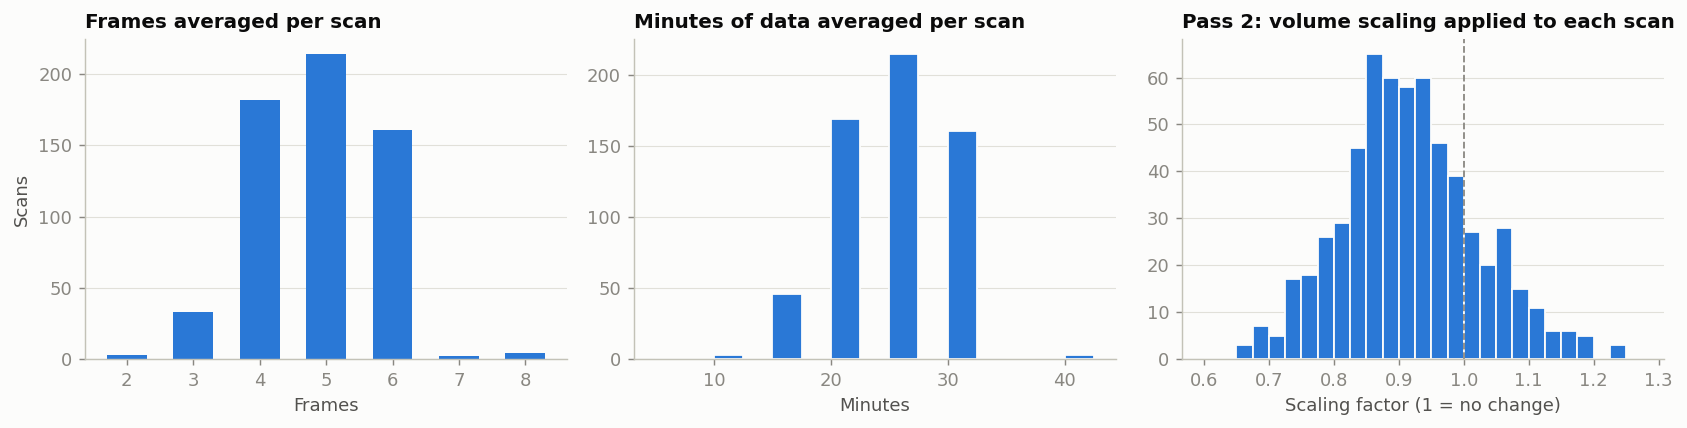
\includegraphics[width=\textwidth]{11_pipeline_qc.png}
\caption{Quality control of the conversion and registration: number of frames and minutes of data averaged per scan, and the volume scaling applied by the affine registration (1 = no change).}
\label{fig:petqc}
\end{figure}

\begin{figure}[H]
\centering
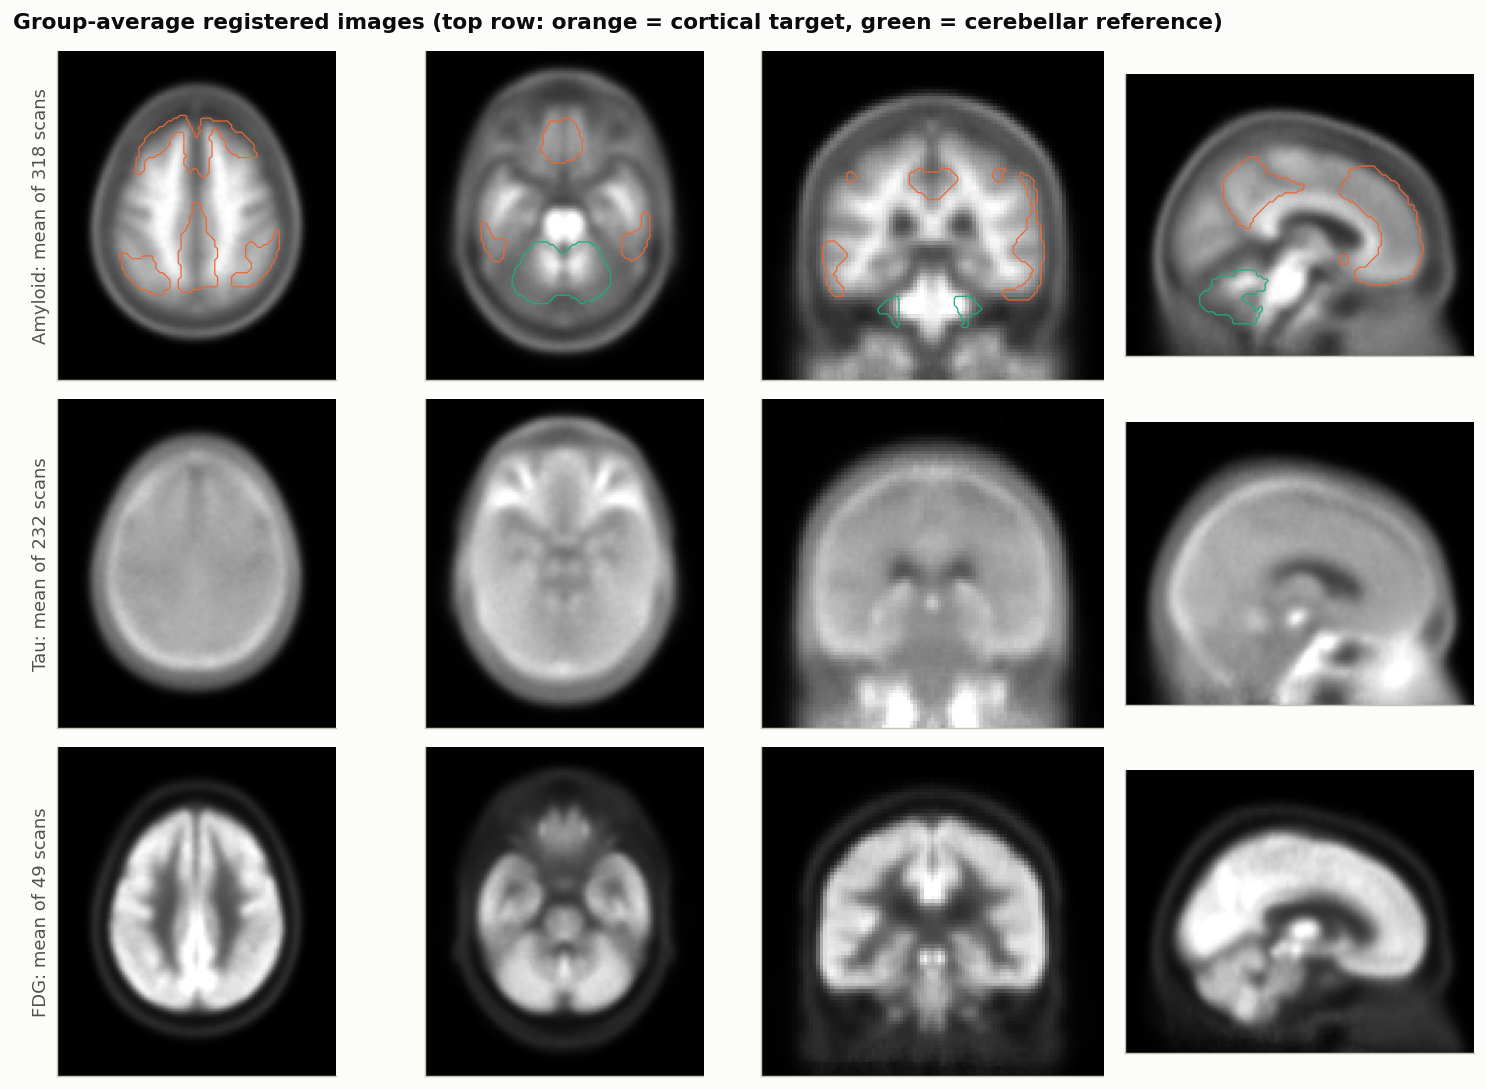
\includegraphics[width=0.92\textwidth]{11_group_average_images.png}
\caption{Average of all registered scans for each tracer class (amyloid, 318 scans; tau, 232; FDG, 49), in axial, coronal and sagittal sections. In the top row the orange outline is the Centiloid cortical target region and the green outline the cerebellar reference region. Only group averages are shown; no individual scan is reproduced.}
\label{fig:petavg}
\end{figure}

\section{Amyloid SUVR from the images}

For each registered amyloid scan, the standardised uptake value ratio was computed as the mean uptake in the cortical target region divided by the mean uptake in the whole cerebellum, using the standard masks of the Centiloid project \cite{klunk2015}:
\begin{equation}
\text{SUVR} = \frac{\frac{1}{|\Omega_{\text{ctx}}|}\sum_{\mathbf{r} \in \Omega_{\text{ctx}}} V(\mathbf{r})}{\frac{1}{|\Omega_{\text{cb}}|}\sum_{\mathbf{r} \in \Omega_{\text{cb}}} V(\mathbf{r})},
\end{equation}
where $\Omega_{\text{ctx}}$ and $\Omega_{\text{cb}}$ are the voxels of the cortical and cerebellar masks. Because the activity scale cancels in the ratio, SUVR does not depend on the injected dose or body weight. NACC's PET core had computed an SUVR for the same scans with a different, MRI-based pipeline in native space. Agreement between the two therefore provides an independent test of the conversion and registration steps. Agreement was summarised by the Pearson and Spearman correlations, the least-squares line $\text{SUVR}_{\text{ours}} = a + b\,\text{SUVR}_{\text{NACC}}$, and the Bland--Altman limits of agreement $\bar{d} \pm 1.96\, s_d$, where $\bar{d}$ and $s_d$ are the mean and standard deviation of the differences $d = \text{SUVR}_{\text{ours}} - \text{SUVR}_{\text{NACC}}$.

\begin{table}[H]
\centering\small
\caption{Agreement between image-derived and NACC amyloid SUVR (318 scans).}
\label{tab:suvr}
\begin{tabular}{@{}lr@{}}
\toprule
Measure & Value \\
\midrule
Pearson correlation & 0.977 \\
Spearman correlation & 0.885 \\
Regression line (ours on NACC) & $-0.16 + 1.10\,x$ \\
Mean difference (ours minus NACC) & $-0.043$ \\
95\% limits of agreement & $-0.18$ to $+0.09$ \\
\bottomrule
\end{tabular}
\end{table}

Agreement was high for every tracer (Pearson $r$ between 0.96 and 0.99 for the four tracers with known identity) and every scanner manufacturer. The lower Spearman correlation reflects the many amyloid-negative scans with similar low values, where small differences change the rank order.

\begin{figure}[H]
\centering
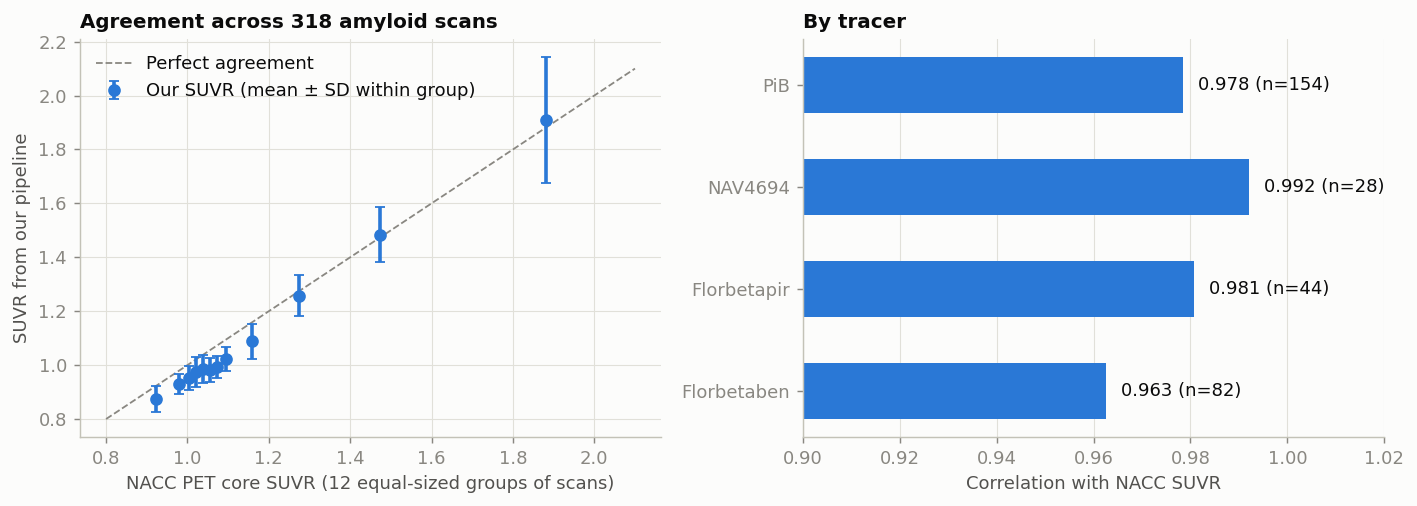
\includegraphics[width=\textwidth]{11_suvr_agreement.png}
\caption{Image-derived amyloid SUVR against the value computed by the NACC PET core for the same scans.}
\label{fig:suvr}
\end{figure}

\section{Amyloid status classification}

Three classifiers of amyloid status were compared on the 292 amyloid scans with a status label from the PET core (84 positive), using five-fold stratified cross-validation so that every scan was predicted by a model that had not seen it: (i) the cortical SUVR alone; (ii) a logistic regression on mean uptake in an $8 \times 8 \times 8$-voxel grid of blocks; and (iii) a small 3D convolutional neural network. The network has four stages of two $3 \times 3 \times 3$ convolutions with instance normalisation and ReLU, each stage halving the resolution, followed by global average pooling, dropout of 0.3 and a linear output, with 494,917 weights in total. Volumes were cropped to the head and resampled to $80 \times 96 \times 80$ voxels. Training used AdamW (learning rate $10^{-3}$, weight decay $10^{-2}$) with a one-cycle schedule, 40 epochs, batches of 8, and augmentation by left--right flips, shifts of up to three voxels and small intensity changes. Because positive scans are the minority, the cross-entropy was weighted,
\begin{equation}
\mathcal{L} = -\frac{1}{n}\sum_i \Big[ w_{+}\, y_i \log \hat{p}_i + (1 - y_i)\log(1 - \hat{p}_i) \Big], \qquad w_{+} = \frac{1 - \bar{y}}{\bar{y}},
\end{equation}
where $\bar{y}$ is the proportion of positive scans in the training folds. The regional logistic model used the mean uptake in each $8 \times 8 \times 8$ block as a feature, with a strong $L_2$ penalty ($C = 0.01$).

\begin{table}[H]
\centering\small
\caption{Amyloid status classification (292 scans, 84 positive, cross-validated).}
\label{tab:cnn}
\begin{tabular}{@{}lr@{}}
\toprule
Method & AUROC \\
\midrule
Cortical SUVR (one number) & 0.982 \\
Regional logistic model & 0.971 \\
3D CNN & 0.960 \\
\bottomrule
\end{tabular}
\end{table}

The single SUVR value performed best (Figure~\ref{fig:cnn}).

\begin{figure}[H]
\centering
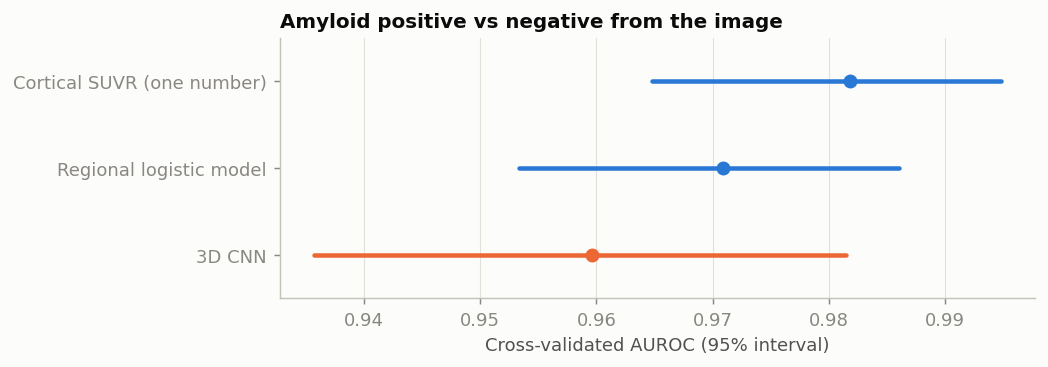
\includegraphics[width=0.85\textwidth]{11_image_models.png}
\caption{Cross-validated AUROC with 95\% bootstrap intervals for the three amyloid-status classifiers.}
\label{fig:cnn}
\end{figure}

 This is expected: the reference label is itself derived by the PET core from a cortical uptake measure, so a scalar SUVR is close to the definition of the label, and a network trained on fewer than 300 scans has little opportunity to improve on it. The experiment shows that the image pipeline supports a working deep-learning model, not that a CNN is preferable for this task.

\section{Grad-CAM}

Gradient-weighted class activation maps \cite{selvaraju2017} were computed for the network and averaged over 72 scans. If $\mathbf{A}^{k}$ is the $k$-th feature map of the last convolutional stage and $s$ the output score, the map is
\begin{equation}
L_{\text{Grad-CAM}} = \operatorname{ReLU}\Big( \sum_k \alpha_k \mathbf{A}^{k} \Big), \qquad
\alpha_k = \frac{1}{Z} \sum_{\mathbf{r}} \frac{\partial s}{\partial A^{k}_{\mathbf{r}}},
\end{equation}
where $Z$ is the number of voxels in the feature map; the map is upsampled to the image size and divided by its maximum. The maps were diffuse: about 96\% of the volume exceeded a quarter of the maximum activation, and only 1.7\% of the most strongly activated voxels lay inside the cortical target region, against 3.8\% expected by chance. The maps therefore do not show that the network attends to the cortical regions where amyloid accumulates, and they are not used as evidence of what the model has learned. Figure~\ref{fig:gradcam} shows the group-average images of amyloid-negative and amyloid-positive scans together with the mean Grad-CAM map: the positive scans show the expected higher cortical uptake, whereas the map is highest at the lower edge of the brain rather than in the cortical target region.

\begin{figure}[H]
\centering
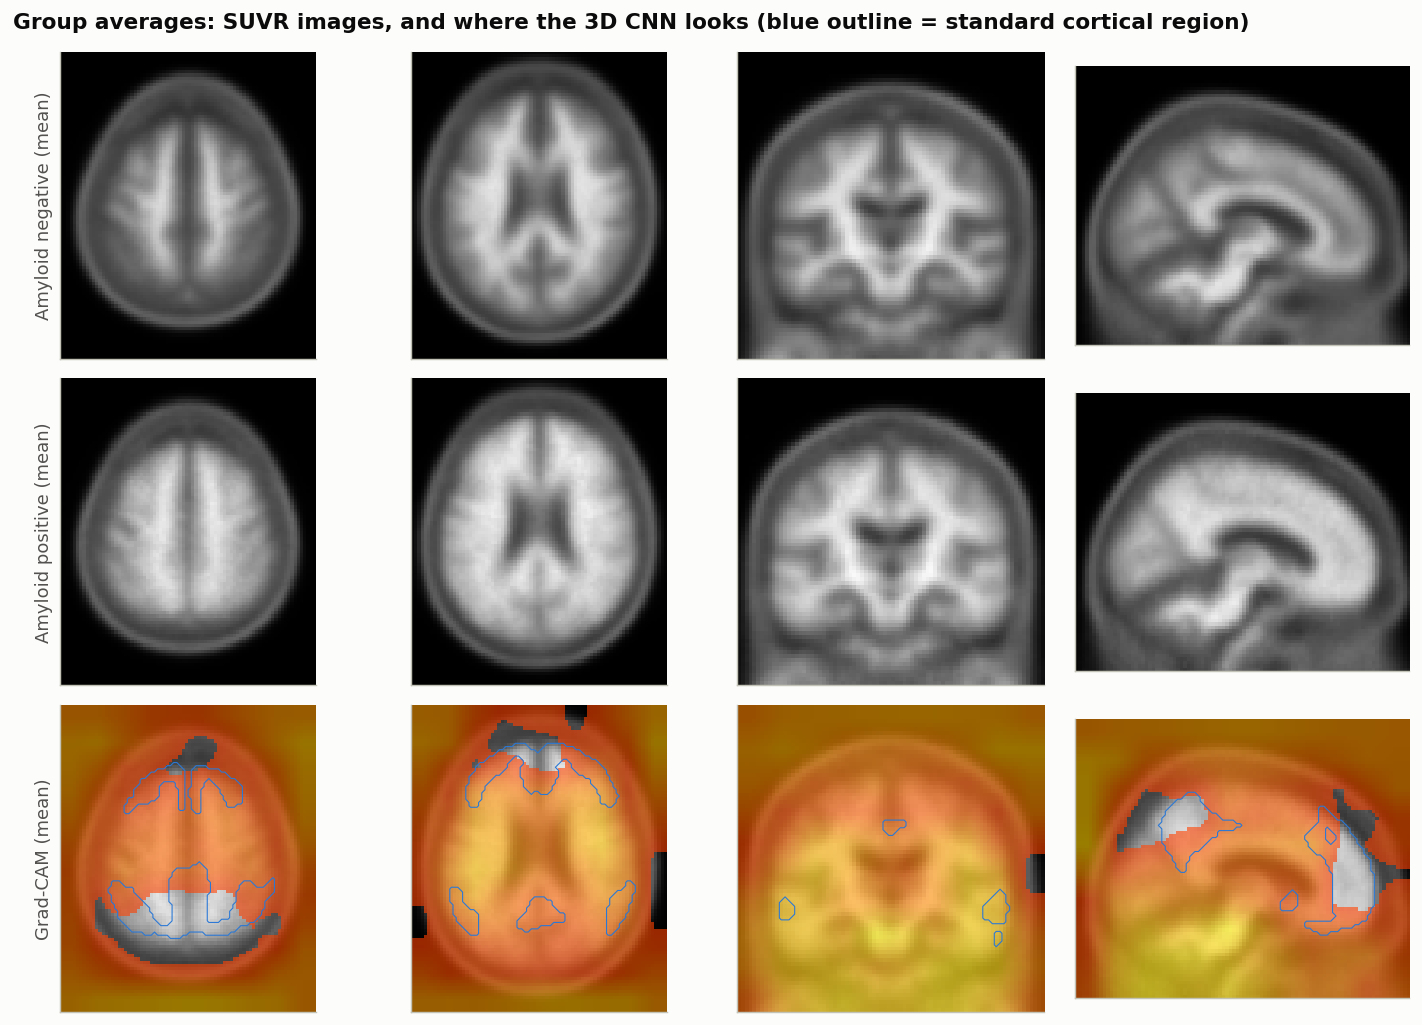
\includegraphics[width=0.92\textwidth]{11_gradcam_mean.png}
\caption{Group-average SUVR images of amyloid-negative and amyloid-positive scans (top two rows) and the mean Grad-CAM map of the 3D CNN (bottom row), in four sections. The blue outline marks the standard cortical target region.}
\label{fig:gradcam}
\end{figure}

\section{Why images are not used to predict dementia}
\label{sec:why_not_images}

Of the 446 participants with an image, about 86\% were cognitively normal at the time of the scan, follow-up after the scan is about two years, and only five later received a dementia diagnosis. No model can learn a reliable pattern from five events, so dementia prediction from images was not attempted. The quantitative PET information that is available for thousands of participants is used instead, through the late-fusion model described in Chapter~\ref{ch:method}.

Two further limitations apply. Registration without an MRI is less precise than the MRI-based pipelines used by PET cores. Tau images were converted and registered but not quantified, because a standard tau target mask comparable to the Centiloid masks was not available.

\chapter{Results}
\label{ch:results}

All results in this chapter are computed on participants who were not used for training: the internal test set (2,286 participants, 332 converters) and the nine held-out centres (4,064 participants, 545 converters). Intervals are 95\% bootstrap intervals. Every number can be traced to a result file in the project repository.

\section{Comparison of models}

\begin{table}[H]
\centering\small
\caption{Discrimination and calibration of the five models.}
\label{tab:models_res}
\begin{tabular}{@{}lccccc@{}}
\toprule
 & \multicolumn{3}{c}{Test set} & \multicolumn{2}{c}{Held-out centres} \\
\cmidrule(lr){2-4}\cmidrule(l){5-6}
Model & AUROC (95\% CI) & AUPRC & Brier & AUROC & Brier \\
\midrule
Logistic regression & 0.936 (0.924--0.949) & 0.721 & 0.066 & 0.945 & 0.060 \\
Random forest & 0.932 (0.919--0.944) & 0.704 & 0.070 & 0.940 & 0.064 \\
XGBoost & 0.938 (0.925--0.948) & 0.713 & 0.066 & 0.946 & 0.059 \\
Multilayer perceptron & 0.938 (0.926--0.949) & 0.721 & 0.066 & 0.946 & 0.059 \\
FT-Transformer & 0.939 (0.927--0.949) & 0.720 & 0.066 & 0.945 & 0.061 \\
\bottomrule
\end{tabular}
\end{table}

The five models perform almost identically, and their confidence intervals overlap almost completely (Table~\ref{tab:models_res}). The deep-learning models did not outperform logistic regression or gradient boosting on these data. For reference, always predicting the training event rate gives a Brier score of 0.124, so all models are substantially better calibrated than a constant prediction.

\begin{figure}[H]
\centering
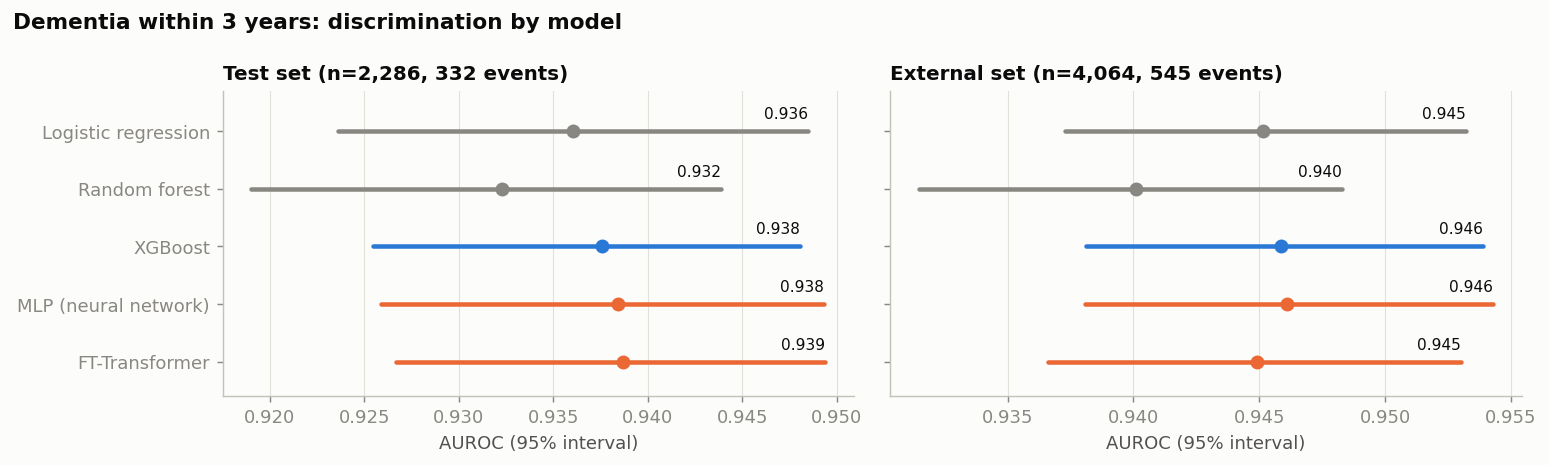
\includegraphics[width=\textwidth]{06_model_comparison.png}
\caption{AUROC and AUPRC of the five models on the test set and the held-out centres.}
\label{fig:models}
\end{figure}

\section{Performance by diagnosis at the index visit}
\label{sec:res_groups}

The cohort combines cognitively normal participants, who rarely convert (1.6\%), with participants with MCI, who often do (41.5\%). Diagnosis alone therefore separates converters from non-converters well: a model given only the diagnosis reaches an AUROC of 0.84. Table~\ref{tab:groups} reports XGBoost separately within each group.

\begin{table}[H]
\centering\small
\caption{XGBoost by diagnosis at the index visit (participants / converters).}
\label{tab:groups}
\begin{tabular}{@{}lcccc@{}}
\toprule
 & \multicolumn{2}{c}{Test set} & \multicolumn{2}{c}{Held-out centres} \\
\cmidrule(lr){2-3}\cmidrule(l){4-5}
Group & $n$ / events & AUROC (95\% CI) & $n$ / events & AUROC (95\% CI) \\
\midrule
All not demented & 2,286 / 332 & 0.937 (0.925--0.948) & 4,064 / 545 & 0.946 (0.938--0.954) \\
Cognitively normal & 1,411 / 24 & 0.884 (0.819--0.936) & 2,624 / 37 & 0.876 (0.823--0.918) \\
MCI & 732 / 289 & 0.835 (0.807--0.862) & 1,291 / 496 & 0.846 (0.824--0.867) \\
\bottomrule
\end{tabular}
\end{table}

Within MCI the AUROC is about 0.84, which is the more informative estimate of how well the model ranks risk among people who are already impaired. Within the cognitively normal group the AUROC is about 0.88, but it rests on only 24 and 37 events and the intervals are wide; with an event rate of 1.6\% the average precision is only 0.15 to 0.19, so most participants flagged as high risk would not convert. Models trained only on normal participants (AUROC 0.876 and 0.881) or only on MCI participants (0.829 and 0.838) gave the same picture, so the group results are not an artefact of mixing the groups during training.

\section{What drives the prediction}

\subsection{Feature categories}

\begin{table}[H]
\centering\small
\caption{Contribution of each feature category (XGBoost, test set unless stated).}
\label{tab:ablation}
\begin{tabular}{@{}lccc@{}}
\toprule
Category & Alone & Gain when added to all others (test) & Gain (held-out centres) \\
\midrule
Cognitive tests & 0.896 & $+0.022$ ($+0.015$ to $+0.029$) & $+0.019$ ($+0.013$ to $+0.024$) \\
Clinical stage (CDR-SB, diagnosis) & 0.897 & $+0.015$ ($+0.007$ to $+0.023$) & $+0.021$ ($+0.015$ to $+0.027$) \\
Demographics & 0.671 & $+0.010$ ($+0.006$ to $+0.015$) & $+0.009$ ($+0.006$ to $+0.013$) \\
Genetics (APOE) & 0.645 & $+0.003$ ($+0.002$ to $+0.004$) & $+0.001$ ($-0.000$ to $+0.002$) \\
Cardiovascular and medical & 0.626 & $+0.001$ ($-0.000$ to $+0.003$) & $+0.001$ ($+0.000$ to $+0.002$) \\
\bottomrule
\end{tabular}
\end{table}

Cognitive tests and clinical stage each reach an AUROC near 0.90 on their own and make the largest unique contributions (Table~\ref{tab:ablation}, Figure~\ref{fig:groups}). Because these two categories overlap, removing either one costs little; removing both together, so that the model has no information about current cognition, lowers the AUROC from 0.937 to 0.746 on the test set (0.744 on the held-out centres). Within the normal and MCI groups the corresponding values are 0.783 and 0.638. The model therefore relies mainly on how impaired a person already is at the index visit. Because all these variables are recorded at the index visit and the outcome occurs later, this is not leakage, but it means the model is best described as estimating short-term progression given the current clinical stage.

\begin{figure}[H]
\centering
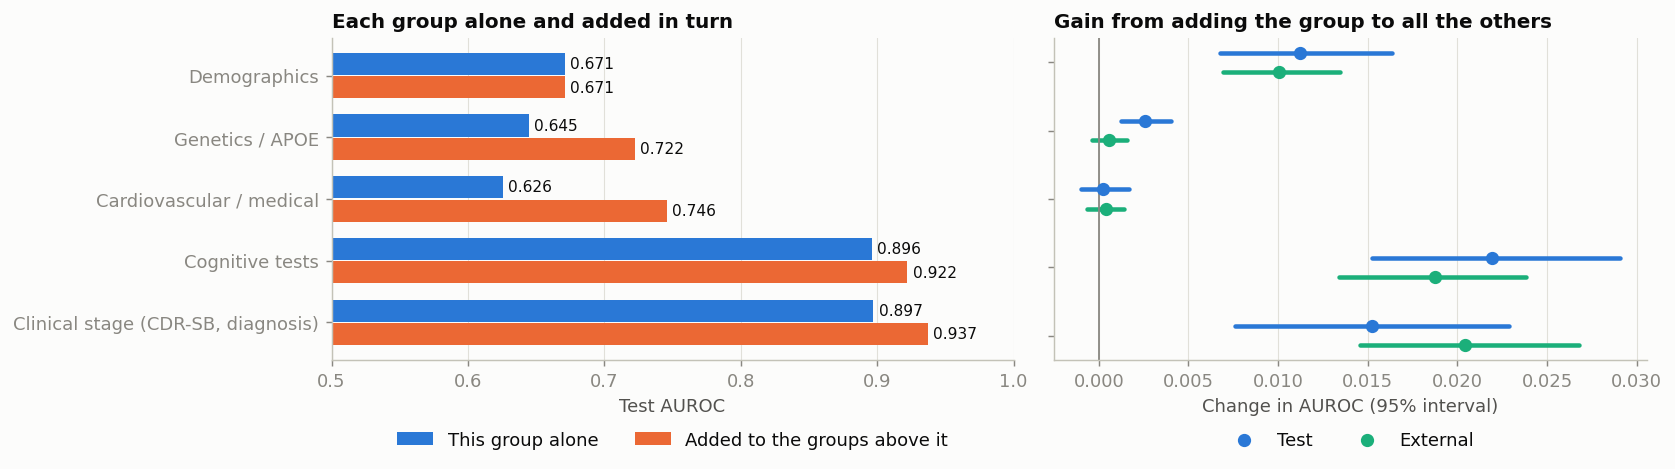
\includegraphics[width=\textwidth]{06_feature_groups.png}
\caption{Left: AUROC of each category alone and added cumulatively. Right: gain in AUROC from adding each category to all the others.}
\label{fig:groups}
\end{figure}

\subsection{Cardiovascular information (research question 1)}

On its own, the cardiovascular category carries some signal (AUROC 0.626). Added to demographics and APOE only, before any cognitive information, it improved the AUROC by 0.024 on the test set (0.011 to 0.039), but by only 0.004 at the held-out centres ($-0.006$ to $0.015$). Once cognitive information is present its contribution falls to about 0.001, with an interval that includes zero on the test set. Within the cognitively normal group the gain was 0.008 on the test set and 0.003 at the held-out centres, with intervals spanning zero. In this cohort and prediction setting, therefore, cardiovascular and medical history added little incremental predictive value beyond current cognitive status. This finding does not imply that vascular health is unimportant for the brain: the participants enter at a median age of 71, mid-life exposure is not observed, and vascular damage that has already occurred is likely to be reflected in the cognitive scores.

\subsection{Shapley explanations}

\begin{table}[H]
\centering\small
\caption{Share of mean absolute SHAP value by category (test set, 2,286 participants).}
\label{tab:shap}
\begin{tabular}{@{}lc@{}}
\toprule
Category & Share \\
\midrule
Clinical stage (CDR-SB, diagnosis) & 40.8\% \\
Cognitive tests & 35.0\% \\
Demographics & 15.5\% \\
Cardiovascular and medical & 5.1\% \\
Genetics & 3.5\% \\
\bottomrule
\end{tabular}
\end{table}

The most important individual features were CDR-SB, MCI status, the memory score, age and the executive score. The ranking was stable across eight bootstrap refits (Spearman correlation with the main model 0.89 to 0.97; 8 to 10 of the top ten features shared). Some associations are not causal: lower BMI was associated with higher predicted risk, which is consistent with weight loss in the years before a dementia diagnosis rather than a protective effect of higher weight.

\section{Cognitive Decline as the Outcome}

Table~\ref{tab:decline} reports the secondary outcome, a rise of at least one point in CDR-SB within three years. The cohort is slightly larger than for dementia (20,355 participants, 5,035 events) because the outcome can be observed in people who decline without reaching dementia.

\begin{table}[H]
\centering\small
\caption{XGBoost for CDR-SB worsening of at least one point within three years (participants / events).}
\label{tab:decline}
\begin{tabular}{@{}lcccc@{}}
\toprule
 & \multicolumn{2}{c}{Test set} & \multicolumn{2}{c}{Held-out centres} \\
\cmidrule(lr){2-3}\cmidrule(l){4-5}
Group & $n$ / events & AUROC (95\% CI) & $n$ / events & AUROC (95\% CI) \\
\midrule
All not demented & 2,375 / 572 & 0.858 (0.841--0.874) & 4,272 / 1,035 & 0.885 (0.875--0.896) \\
Cognitively normal & 1,459 / 129 & 0.760 (0.714--0.805) & 2,690 / 215 & 0.831 (0.806--0.856) \\
MCI & 766 / 399 & 0.748 (0.712--0.779) & 1,411 / 774 & 0.749 (0.723--0.776) \\
\bottomrule
\end{tabular}
\end{table}

Decline is harder to predict than dementia, as expected for an outcome that includes small changes in a rating scale. The cognitively normal group is much better represented here (129 and 215 events instead of 24 and 37), so the estimate of 0.76 to 0.83 in that group is more reliable than the corresponding dementia result. Logistic regression gave almost the same result (0.854 and 0.883). The pattern of contributions matched the dementia outcome: cognitive tests made the largest unique contribution ($+0.029$ on the test set), and the cardiovascular category added nothing measurable ($+0.0004$, interval $-0.003$ to $+0.003$; held-out centres $0.000$).

\subsection{Predicted Change in CDR-SB}

For the 1,863 test participants and 3,231 held-out participants with a visit near the three-year mark, the mean change in CDR-SB was 0.48 and 0.63 points, and three quarters showed no change or an improvement. The regression model reduced the mean absolute error from 0.69 (predicting no change) to 0.60 on the test set and from 0.83 to 0.72 at the held-out centres, with $R^2$ of 0.23 and 0.18 and a Spearman correlation of 0.45. Within MCI the error fell from 1.90 to 1.59 points. Within cognitively normal participants, whose scores rarely change, the model was no better than predicting no change (0.17 against 0.17). The progression estimate is therefore informative for people who are already impaired and adds little for people who are not.

\section{Modality-Encoder Fusion Network}

The fusion network reached an AUROC of 0.934 (0.920--0.946) on the test set and 0.943 (0.935--0.951) at the held-out centres for dementia, against 0.937 and 0.946 for XGBoost; within MCI 0.831 and 0.837, and within cognitively normal participants 0.846 and 0.874. Its progression head reduced the mean absolute error from 0.72 to 0.65 on the test set. With modalities removed it behaved like the modality-dropout XGBoost model: without any cognitive information its AUROC was 0.72 and its Brier score 0.114, close to the specialist value.

The attention weights, intended as an explanation of how much the network relied on each modality, were nearly equal: between 18\% and 21\% for every modality, on both evaluation sets and in every diagnostic group. They stayed almost equal even when the cognitive modalities were missing, because the learned missing tokens themselves carry the information. The attention weights therefore do not reveal which modality drives a prediction, in line with the wider observation that attention weights are not reliable explanations. The ablation results and SHAP values, which show that cognitive information dominates, remain the explanations used in this work. The fusion network demonstrates that the proposed architecture works and copes with missing modalities, but it offers no gain in accuracy over gradient-boosted trees on these data.

\section{Longitudinal information}

On landmark visits preceded by at least two earlier visits (test: 1,205 participants, 166 events; held-out centres: 2,254 participants, 326 events), adding the visit history produced only small changes (Table~\ref{tab:long}).

\begin{table}[H]
\centering\small
\caption{Effect of earlier visits (paired gain over the landmark-only model).}
\label{tab:long}
\begin{tabular}{@{}lcc@{}}
\toprule
Model & Test AUROC (gain) & Held-out AUROC (gain) \\
\midrule
XGBoost, landmark visit only & 0.919 & 0.953 \\
XGBoost with trajectory features & 0.922 ($+0.003$; $-0.006$ to $+0.011$) & 0.956 ($+0.003$; $-0.001$ to $+0.007$) \\
GRU over the visit sequence & 0.920 ($+0.000$; $-0.011$ to $+0.010$) & 0.958 ($+0.005$; $+0.001$ to $+0.008$) \\
\bottomrule
\end{tabular}
\end{table}

When current scores are known, the path that led to them adds little for a three-year prediction. This does not show that longitudinal modelling is of no value; a longer horizon, an earlier disease stage or more frequent measurement could give a different result.

\section{PET measures (research question 2)}
\label{sec:res_pet}

On its own, amyloid status is strongly associated with progression: among participants with MCI in the held-out sets, about 34\% of amyloid-positive participants received a dementia diagnosis within two years, compared with about 7\% of amyloid-negative participants (36\% and 9\% under the strict scan-matching rule). Added to the clinical model, however, the PET measures did not produce a clear improvement under either matching rule. For example, with strict matching and a three-year horizon, the AUROC at the held-out centres was 0.939 without and 0.946 with amyloid (191 participants, 27 events; paired gain $-0.007$ to $+0.024$). The final late-fusion model scored 0.964 against 0.944 for the clinical model on 243 held-out scanned participants with 33 events, a gain of 0.020 whose interval ($-0.009$ to $+0.066$) includes zero. A modest benefit cannot be excluded, but it could not be demonstrated with the follow-up currently available.

\section{Validation}

\subsection{Subgroups}

\begin{table}[H]
\centering\small
\caption{XGBoost AUROC by subgroup.}
\label{tab:subgroups}
\begin{tabular}{@{}lcc@{}}
\toprule
Subgroup & Test (n / events) & Held-out centres (n / events) \\
\midrule
Female & 0.950 (1,338 / 162) & 0.947 (2,507 / 272) \\
Male & 0.919 (948 / 170) & 0.941 (1,557 / 273) \\
Age under 65 & 0.976 (467 / 46) & 0.958 (1,067 / 56) \\
Age 65--74 & 0.952 (963 / 99) & 0.956 (1,463 / 191) \\
Age 75--84 & 0.904 (732 / 157) & 0.937 (1,044 / 191) \\
Age 85 and over & 0.852 (124 / 30) & 0.888 (490 / 107) \\
White & 0.933 (1,813 / 273) & 0.943 (3,347 / 499) \\
Black & 0.948 (304 / 31) & 0.951 (471 / 26) \\
Education 12 years or less & 0.926 (400 / 92) & 0.920 (744 / 137) \\
Education over 16 years & 0.951 (937 / 112) & 0.960 (1,551 / 188) \\
APOE $\varepsilon$4 carrier & 0.915 (762 / 150) & 0.933 (1,402 / 277) \\
\bottomrule
\end{tabular}
\end{table}

Discrimination was similar across sex, race and education. It was lower in the oldest participants and in APOE $\varepsilon$4 carriers, both groups with a higher baseline risk.

\subsection{Calibration and clinical usefulness}

On the test set the mean predicted risk (14.5\%) equalled the observed rate (14.5\%), with a calibration slope of 1.01 and intercept of 0.009. At the held-out centres the model over-predicted slightly (15.0\% predicted, 13.4\% observed; slope 1.10). Using a risk threshold of 20\%, the model flagged 22\% of test participants with a sensitivity of 83\%, specificity of 88\%, positive predictive value of 55\% and negative predictive value of 97\% (held-out centres: 90\%, 87\%, 52\% and 98\%). Decision curve analysis showed a higher net benefit than treating everyone or no one across all thresholds examined, from 2\% to 60\%, on both evaluation sets.

\section{Missing information}

\begin{table}[H]
\centering\small
\caption{Brier score when categories are missing (test set; lower is better).}
\label{tab:dropout}
\begin{tabular}{@{}lccc@{}}
\toprule
Available information & Standard model & Modality dropout & Specialist model \\
\midrule
Everything & 0.066 & 0.067 & 0.066 \\
No cognitive tests & 0.082 & 0.077 & 0.080 \\
No clinical stage & 0.185 & 0.076 & 0.074 \\
No cognitive information at all & 0.441 & 0.115 & 0.111 \\
Demographics only & 0.444 & 0.120 & 0.118 \\
\bottomrule
\end{tabular}
\end{table}

A standard model given missing inputs at prediction time produced badly calibrated risks when cognitive information was absent, worse than predicting the base rate (Brier 0.124). The model trained with modality dropout stayed close to a specialist model retrained for each situation (Table~\ref{tab:dropout}), with almost no loss when all information is present. This model is used in the clinician interface.

\section{Sensitivity analyses}
\label{sec:res_sens}

\textbf{Censored participants.} A Cox model fitted on all eligible participants, including those followed for less than three years, reached a concordance index of 0.891 on the test set and 0.903 at the held-out centres. Removing the cardiovascular category changed the concordance by 0.001 ($-0.001$ to $0.003$) and 0.000 ($-0.001$ to $0.002$). Hazard ratios per standard deviation were 1.37 for CDR-SB, 0.76 for the memory score, 1.40 for age and 1.20 for each APOE $\varepsilon$4 allele, while hypertension (0.995, 0.953--1.038), diabetes and stroke had hazard ratios close to one.

\textbf{Reversed diagnoses.} A clinical diagnosis can be revised. Of the 2,818 converters, 217 (7.7\%) were recorded as not demented at a later visit. Excluding them, XGBoost reached an AUROC of 0.947 on the test set and 0.950 at the held-out centres (MCI: 0.839 and 0.851). The conclusions do not depend on reversed diagnoses.

\textbf{Variables close to the diagnosis.} Adding the daily-function questionnaire, independence, memory complaints and Alzheimer's medication increased the AUROC by 0.006 on the test set and 0.005 at the held-out centres. These variables were therefore left out of the main model with little loss of accuracy.

\chapter{System Design}
\label{ch:system}

The models are packaged as a research prototype for a clinician: an interface for entering a patient's information and seeing a risk estimate with its explanation, and an evidence assistant that answers questions from a fixed library of published papers. The prototype is not intended for clinical use and states this on every screen.

\section{Architecture}

\begin{table}[H]
\centering\small
\caption{Components of the prototype.}
\label{tab:components}
\begin{tabularx}{\textwidth}{@{}lY@{}}
\toprule
Component & Role \\
\midrule
Inference module (\texttt{scripts/inference.py}) & Converts raw entries into the 48 model features (for example a MoCA score into the global $z$-score), runs the modality-dropout model and the PET fusion model, computes SHAP values and checks the plausibility of the entries \\
API (\texttt{app/api.py}, FastAPI) & Serves the form definition, predictions and evidence-assistant answers \\
Interface (\texttt{app/web}, React) & The form and the results \\
Evidence assistant (\texttt{scripts/rag.py}) & Retrieval, guardrails and answer generation \\
\bottomrule
\end{tabularx}
\end{table}

\section{Input form}

The form is generated from the list of features the model was trained on, so it asks for exactly those inputs and nothing else. It has one section per category: demographics (required), cardiovascular history and measurements, the clinician's assessment (cognitive status and CDR-SB), test scores, genetics, and PET. The clinician marks each optional section as available or not. Empty fields are passed to the model as missing values; no default values are substituted. For each test the form shows the expected score of a healthy person of the same age, sex and education.

\section{Output}

The interface reports the estimated three-year risk next to the observed three-year conversion rate of training participants in the same age group and with the same cognitive status, which gives the clinician an empirical reference point. It lists which categories were used and which were missing, and shows the SHAP contributions of each category and of the most influential individual items. When no cognitive information is available, it states that the estimate is little more than an age-based average.

\section{Plain-Language Report}

On request, the interface writes a short report for the clinician. It has five parts: a summary of the estimated risk next to the observed conversion rate of similar participants; the main reasons, built from the largest positive and negative SHAP contributions and phrased in plain terms (for example, ``memory tests below expected for age, sex and education''); the reliability of the estimate, listing missing categories and any plausibility warnings; one or two quoted passages from the evidence library on the factors that drove the estimate, each with its source; and a fixed statement of the limits of the estimate. The report is assembled from templates filled with the person's own numbers, and the evidence is quoted rather than generated, so the report cannot state anything that the model or the literature did not provide.

\section{Plausibility checks}

Contradictory entries can produce estimates that look precise but are meaningless. For example, a MoCA score of 0 entered together with a status of ``normal'' and a CDR-SB of 0 yields a low risk, because the model gives most weight to the clinician's rating. The interface therefore checks the entries against the ranges observed in training data before showing a result. Entries that contradict each other (test scores below the first percentile of cognitively normal participants combined with a normal status; a CDR-SB above the 99th percentile for the stated status; systolic pressure not above diastolic; implausible smoking duration) are flagged and the estimate is marked as unreliable. Unusual but possible entries (age outside the 1st to 99th percentile of the training cohort, very low education, discordant PET values) generate a note.

\section{Behaviour checks}

Twenty-eight automated checks test the deployed model through the same code path as the interface. They confirm that the form covers every trained feature and no other; that typical cognitively normal, impaired and MCI cases receive plausible, correctly ordered estimates (0.6\%, 4.0\% and 60.8\%); that a worse CDR-SB, a worse cognitive status, lower test scores, more APOE $\varepsilon$4 alleles or more behavioural symptoms never lower the estimate; that contradictory entries are flagged; and that missing categories are reported. Twenty-seven checks pass. The remaining check compares predicted and observed risk within age and diagnosis groups on held-out data: ten of eleven groups agree within seven percentage points, but for participants with MCI under the age of 65 the model predicts 35\% against an observed 27\%. This over-prediction is reported as a known limitation.

\section{Evidence assistant}

The evidence assistant is a retrieval-augmented generation system \cite{lewis2020}. Its library consists of eleven open-access papers on dementia risk factors, vascular contributions, APOE, amyloid and tau PET and diagnostic criteria, divided into 447 passages. For a question, two rankings are computed, one by semantic similarity of sentence embeddings \cite{reimers2019} and one by BM25 keyword relevance \cite{robertson2009}, and merged by reciprocal rank fusion \cite{cormack2009}. If the best semantic similarity is below a fixed threshold (0.35), the assistant reports that the library contains no evidence on the question. Otherwise a small instruction-tuned language model running locally writes an answer from the retrieved passages with numbered citations; if the answer does not cite the passages correctly, the assistant quotes them directly instead. Questions asking for advice about a particular person are answered with a notice that the system cannot give individual medical advice, followed by general published information only. No data leave the machine.

\begin{table}[H]
\centering\small
\caption{Evaluation of the evidence assistant (52 questions).}
\label{tab:rag}
\begin{tabular}{@{}lc@{}}
\toprule
Measure & Result \\
\midrule
Correct source ranked first (hybrid retrieval) & 32 of 32 \\
Correct source ranked first (embeddings only / BM25 only) & 28 of 32 / 31 of 32 \\
Personal-advice questions flagged & 8 of 8 \\
General questions wrongly flagged as advice & 0 of 6 \\
Out-of-scope questions declined & 6 of 6 \\
Answers written with valid citations by the language model & 22\% (otherwise quoted) \\
\bottomrule
\end{tabular}
\end{table}

These results should be read with care. The library is small and the test questions were written by the project team, so retrieval is an easy test. The local language model is small and produced a properly cited answer for only about one question in five; direct quotation is the fallback and is the safer behaviour for medical content.

\chapter{Verification and Reproducibility}
\label{ch:verification}

Clinical prediction studies are vulnerable to subtle errors that inflate performance: the same person in training and test data, information from the future in the features, mislabelled outcomes, or reported numbers that do not match the saved predictions. A separate verification program (\texttt{scripts/verify\_results.py}) was written to test for these errors independently of the main pipeline. Each check recomputes a quantity in a second, simpler way or tests a property that must hold if the pipeline is correct.

\section{Checks}

\begin{table}[H]
\centering\small
\caption{Independent verification checks and their results.}
\label{tab:checks}
\begin{tabularx}{\textwidth}{@{}lYY@{}}
\toprule
Group & Check & Result \\
\midrule
A & Raw files unchanged since the first audit; all 599 image folders present & Pass \\
B & No participant in more than one partition; no held-out centre in the training data; saved split matches the modelling table & 0 participants and 0 centres shared \\
C & Features at the first and third visit are identical when all later visits are deleted before the features are built & Identical for 1,500 participants $\times$ 67 features at each visit \\
C & No PET value is newer than the visit at which it is used & 0 of 1,481 amyloid and 713 tau values \\
D & Outcome labels recomputed with an independent implementation & 0 disagreements in 11,403 visits \\
D & No eligible index visit has a dementia diagnosis & 0 of 134,943 \\
E & With shuffled outcome labels, a retrained model falls to chance & AUROC 0.508 \\
F & Reported AUROC values recomputed from the saved predictions & Largest difference 0 over 5 models and 2 evaluation sets \\
F & Cohort sizes in the reports match the modelling table & Match \\
G & Retraining from scratch with a new seed reproduces the result & Test 0.937, held-out 0.946 (reported 0.938, 0.946) \\
G & Gain from the cardiovascular category with a fresh seed & $+0.0016$ \\
H & Cohort flow and PET index counts in the reports match the data & Match \\
\bottomrule
\end{tabularx}
\end{table}

All seventeen checks passed on the final pipeline (re-run on 23 October 2026).

\section{Errors found and corrected}

The checks found two genuine errors in an earlier version of the pipeline, both of which used information that would not have been available at the time of prediction:

\begin{enumerate}
\item Missing education and race at an early visit had been filled in from a later visit for about 0.1\% of participants. Fixed characteristics are now carried forward only.
\item PET scans had been matched to the nearest visit, which for many participants was a visit a few weeks before the scan. A scan is now used only at a visit on or after its acquisition date.
\end{enumerate}

After both corrections every model was retrained and every result regenerated. The main results changed only in the third decimal place. Earlier outputs were retained for comparison.

\section{Reproducibility}

All random seeds are fixed (2026 for the split, 0 to 2 for model training). Package versions are recorded in \texttt{requirements.txt}. The pipeline is run by a fixed sequence of scripts documented in the repository; given the NACC data, it regenerates every table in this thesis. Participant-level data and trained models are not distributed, in accordance with the data use agreement; all shared outputs are aggregates, and each report is checked automatically for participant identifiers before it is written.


\chapter{Discussion and Limitations}
\textit{To be written (see docs/project\_audit.md).}

\chapter{Conclusion and Future Work}
\textit{To be written.}

\bibliographystyle{IEEEtranN}
\bibliography{references}
\end{document}
